% Options for packages loaded elsewhere
\PassOptionsToPackage{unicode}{hyperref}
\PassOptionsToPackage{hyphens}{url}
%
\documentclass[
]{article}
\usepackage{lmodern}
\usepackage{amssymb,amsmath}
\usepackage{ifxetex,ifluatex}
\ifnum 0\ifxetex 1\fi\ifluatex 1\fi=0 % if pdftex
  \usepackage[T1]{fontenc}
  \usepackage[utf8]{inputenc}
  \usepackage{textcomp} % provide euro and other symbols
\else % if luatex or xetex
  \usepackage{unicode-math}
  \defaultfontfeatures{Scale=MatchLowercase}
  \defaultfontfeatures[\rmfamily]{Ligatures=TeX,Scale=1}
\fi
% Use upquote if available, for straight quotes in verbatim environments
\IfFileExists{upquote.sty}{\usepackage{upquote}}{}
\IfFileExists{microtype.sty}{% use microtype if available
  \usepackage[]{microtype}
  \UseMicrotypeSet[protrusion]{basicmath} % disable protrusion for tt fonts
}{}
\makeatletter
\@ifundefined{KOMAClassName}{% if non-KOMA class
  \IfFileExists{parskip.sty}{%
    \usepackage{parskip}
  }{% else
    \setlength{\parindent}{0pt}
    \setlength{\parskip}{6pt plus 2pt minus 1pt}}
}{% if KOMA class
  \KOMAoptions{parskip=half}}
\makeatother
\usepackage{xcolor}
\IfFileExists{xurl.sty}{\usepackage{xurl}}{} % add URL line breaks if available
\IfFileExists{bookmark.sty}{\usepackage{bookmark}}{\usepackage{hyperref}}
\hypersetup{
  pdftitle={Predicting Ames, Iowa Housing Price},
  pdfauthor={Alex Navarro},
  hidelinks,
  pdfcreator={LaTeX via pandoc}}
\urlstyle{same} % disable monospaced font for URLs
\usepackage[margin=1in]{geometry}
\usepackage{color}
\usepackage{fancyvrb}
\newcommand{\VerbBar}{|}
\newcommand{\VERB}{\Verb[commandchars=\\\{\}]}
\DefineVerbatimEnvironment{Highlighting}{Verbatim}{commandchars=\\\{\}}
% Add ',fontsize=\small' for more characters per line
\usepackage{framed}
\definecolor{shadecolor}{RGB}{248,248,248}
\newenvironment{Shaded}{\begin{snugshade}}{\end{snugshade}}
\newcommand{\AlertTok}[1]{\textcolor[rgb]{0.94,0.16,0.16}{#1}}
\newcommand{\AnnotationTok}[1]{\textcolor[rgb]{0.56,0.35,0.01}{\textbf{\textit{#1}}}}
\newcommand{\AttributeTok}[1]{\textcolor[rgb]{0.77,0.63,0.00}{#1}}
\newcommand{\BaseNTok}[1]{\textcolor[rgb]{0.00,0.00,0.81}{#1}}
\newcommand{\BuiltInTok}[1]{#1}
\newcommand{\CharTok}[1]{\textcolor[rgb]{0.31,0.60,0.02}{#1}}
\newcommand{\CommentTok}[1]{\textcolor[rgb]{0.56,0.35,0.01}{\textit{#1}}}
\newcommand{\CommentVarTok}[1]{\textcolor[rgb]{0.56,0.35,0.01}{\textbf{\textit{#1}}}}
\newcommand{\ConstantTok}[1]{\textcolor[rgb]{0.00,0.00,0.00}{#1}}
\newcommand{\ControlFlowTok}[1]{\textcolor[rgb]{0.13,0.29,0.53}{\textbf{#1}}}
\newcommand{\DataTypeTok}[1]{\textcolor[rgb]{0.13,0.29,0.53}{#1}}
\newcommand{\DecValTok}[1]{\textcolor[rgb]{0.00,0.00,0.81}{#1}}
\newcommand{\DocumentationTok}[1]{\textcolor[rgb]{0.56,0.35,0.01}{\textbf{\textit{#1}}}}
\newcommand{\ErrorTok}[1]{\textcolor[rgb]{0.64,0.00,0.00}{\textbf{#1}}}
\newcommand{\ExtensionTok}[1]{#1}
\newcommand{\FloatTok}[1]{\textcolor[rgb]{0.00,0.00,0.81}{#1}}
\newcommand{\FunctionTok}[1]{\textcolor[rgb]{0.00,0.00,0.00}{#1}}
\newcommand{\ImportTok}[1]{#1}
\newcommand{\InformationTok}[1]{\textcolor[rgb]{0.56,0.35,0.01}{\textbf{\textit{#1}}}}
\newcommand{\KeywordTok}[1]{\textcolor[rgb]{0.13,0.29,0.53}{\textbf{#1}}}
\newcommand{\NormalTok}[1]{#1}
\newcommand{\OperatorTok}[1]{\textcolor[rgb]{0.81,0.36,0.00}{\textbf{#1}}}
\newcommand{\OtherTok}[1]{\textcolor[rgb]{0.56,0.35,0.01}{#1}}
\newcommand{\PreprocessorTok}[1]{\textcolor[rgb]{0.56,0.35,0.01}{\textit{#1}}}
\newcommand{\RegionMarkerTok}[1]{#1}
\newcommand{\SpecialCharTok}[1]{\textcolor[rgb]{0.00,0.00,0.00}{#1}}
\newcommand{\SpecialStringTok}[1]{\textcolor[rgb]{0.31,0.60,0.02}{#1}}
\newcommand{\StringTok}[1]{\textcolor[rgb]{0.31,0.60,0.02}{#1}}
\newcommand{\VariableTok}[1]{\textcolor[rgb]{0.00,0.00,0.00}{#1}}
\newcommand{\VerbatimStringTok}[1]{\textcolor[rgb]{0.31,0.60,0.02}{#1}}
\newcommand{\WarningTok}[1]{\textcolor[rgb]{0.56,0.35,0.01}{\textbf{\textit{#1}}}}
\usepackage{graphicx,grffile}
\makeatletter
\def\maxwidth{\ifdim\Gin@nat@width>\linewidth\linewidth\else\Gin@nat@width\fi}
\def\maxheight{\ifdim\Gin@nat@height>\textheight\textheight\else\Gin@nat@height\fi}
\makeatother
% Scale images if necessary, so that they will not overflow the page
% margins by default, and it is still possible to overwrite the defaults
% using explicit options in \includegraphics[width, height, ...]{}
\setkeys{Gin}{width=\maxwidth,height=\maxheight,keepaspectratio}
% Set default figure placement to htbp
\makeatletter
\def\fps@figure{htbp}
\makeatother
\setlength{\emergencystretch}{3em} % prevent overfull lines
\providecommand{\tightlist}{%
  \setlength{\itemsep}{0pt}\setlength{\parskip}{0pt}}
\setcounter{secnumdepth}{-\maxdimen} % remove section numbering

\title{Predicting Ames, Iowa Housing Price}
\author{Alex Navarro}
\date{10/27/2021}

\begin{document}
\maketitle

\hypertarget{exploratory-data-analysis}{%
\section{Exploratory Data Analysis}\label{exploratory-data-analysis}}

\begin{Shaded}
\begin{Highlighting}[]
\CommentTok{# Set Seed to Save Models:}
\KeywordTok{set.seed}\NormalTok{(}\DecValTok{1}\NormalTok{)}

\CommentTok{# check head of dataframe:}
\KeywordTok{head}\NormalTok{(data, }\DataTypeTok{n =} \DecValTok{10}\NormalTok{)}
\end{Highlighting}
\end{Shaded}

\begin{verbatim}
##    MS.Zoning Lot.Frontage Lot.Area Street Alley Lot.Shape Land.Contour
## 1         RL          141    31770   Pave  None       IR1          Lvl
## 2         RH           80    11622   Pave  None       Reg          Lvl
## 3         RL           81    14267   Pave  None       IR1          Lvl
## 4         RL           93    11160   Pave  None       Reg          Lvl
## 5         RL           74    13830   Pave  None       IR1          Lvl
## 6         RL           78     9978   Pave  None       IR1          Lvl
## 7         RL           41     4920   Pave  None       Reg          Lvl
## 8         RL           43     5005   Pave  None       IR1          HLS
## 9         RL           39     5389   Pave  None       IR1          Lvl
## 10        RL           60     7500   Pave  None       Reg          Lvl
##    Lot.Config Land.Slope Condition.1 Condition.2 Bldg.Type House.Style
## 1      Corner        Gtl        Norm        Norm      1Fam      1Story
## 2      Inside        Gtl       Feedr        Norm      1Fam      1Story
## 3      Corner        Gtl        Norm        Norm      1Fam      1Story
## 4      Corner        Gtl        Norm        Norm      1Fam      1Story
## 5      Inside        Gtl        Norm        Norm      1Fam      2Story
## 6      Inside        Gtl        Norm        Norm      1Fam      2Story
## 7      Inside        Gtl        Norm        Norm    TwnhsE      1Story
## 8      Inside        Gtl        Norm        Norm    TwnhsE      1Story
## 9      Inside        Gtl        Norm        Norm    TwnhsE      1Story
## 10     Inside        Gtl        Norm        Norm      1Fam      2Story
##    Overall.Qual Overall.Cond Year.Built Year.Remod.Add Roof.Style Roof.Matl
## 1             6            5       1960           1960        Hip   CompShg
## 2             5            6       1961           1961      Gable   CompShg
## 3             6            6       1958           1958        Hip   CompShg
## 4             7            5       1968           1968        Hip   CompShg
## 5             5            5       1997           1998      Gable   CompShg
## 6             6            6       1998           1998      Gable   CompShg
## 7             8            5       2001           2001      Gable   CompShg
## 8             8            5       1992           1992      Gable   CompShg
## 9             8            5       1995           1996      Gable   CompShg
## 10            7            5       1999           1999      Gable   CompShg
##    Exterior.1st Exterior.2nd Mas.Vnr.Type Mas.Vnr.Area Exter.Qual Exter.Cond
## 1       BrkFace      Plywood        Stone          112         TA         TA
## 2       VinylSd      VinylSd         None            0         TA         TA
## 3          Wood         wood      BrkFace          108         TA         TA
## 4       BrkFace      BrkFace         None            0         Gd         TA
## 5       VinylSd      VinylSd         None            0         TA         TA
## 6       VinylSd      VinylSd      BrkFace           20         TA         TA
## 7       CemntBd      CmentBd         None            0         Gd         TA
## 8       HdBoard      HdBoard         None            0         Gd         TA
## 9       CemntBd      CmentBd         None            0         Gd         TA
## 10      VinylSd      VinylSd         None            0         TA         TA
##    Foundation Bsmt.Qual Bsmt.Cond Bsmt.Exposure BsmtFin.Type.1 BsmtFin.SF.1
## 1      CBlock        TA        Gd            Gd            BLQ          639
## 2      CBlock        TA        TA            No            Rec          468
## 3      CBlock        TA        TA            No            ALQ          923
## 4      CBlock        TA        TA            No            ALQ         1065
## 5       PConc        Gd        TA            No            GLQ          791
## 6       PConc        TA        TA            No            GLQ          602
## 7       PConc        Gd        TA            Mn            GLQ          616
## 8       PConc        Gd        TA            No            ALQ          263
## 9       PConc        Gd        TA            No            GLQ         1180
## 10      PConc        TA        TA            No            Unf            0
##    BsmtFin.Type.2 BsmtFin.SF.2 Bsmt.Unf.SF Total.Bsmt.SF Heating Heating.QC
## 1             Unf            0         441          1080     Gas         Fa
## 2             LwQ          144         270           882     Gas         TA
## 3             Unf            0         406          1329     Gas         TA
## 4             Unf            0        1045          2110     Gas         Ex
## 5             Unf            0         137           928     Gas         Gd
## 6             Unf            0         324           926     Gas         Ex
## 7             Unf            0         722          1338     Gas         Ex
## 8             Unf            0        1017          1280     Gas         Ex
## 9             Unf            0         415          1595     Gas         Ex
## 10            Unf            0         994           994     Gas         Gd
##    Central.Air Electrical X1st.Flr.SF X2nd.Flr.SF Low.Qual.Fin.SF Gr.Liv.Area
## 1            Y      SBrkr        1656           0               0        1656
## 2            Y      SBrkr         896           0               0         896
## 3            Y      SBrkr        1329           0               0        1329
## 4            Y      SBrkr        2110           0               0        2110
## 5            Y      SBrkr         928         701               0        1629
## 6            Y      SBrkr         926         678               0        1604
## 7            Y      SBrkr        1338           0               0        1338
## 8            Y      SBrkr        1280           0               0        1280
## 9            Y      SBrkr        1616           0               0        1616
## 10           Y      SBrkr        1028         776               0        1804
##    Bsmt.Full.Bath Bsmt.Half.Bath Full.Bath Half.Bath Bedroom.AbvGr
## 1               1              0         1         0             3
## 2               0              0         1         0             2
## 3               0              0         1         1             3
## 4               1              0         2         1             3
## 5               0              0         2         1             3
## 6               0              0         2         1             3
## 7               1              0         2         0             2
## 8               0              0         2         0             2
## 9               1              0         2         0             2
## 10              0              0         2         1             3
##    Kitchen.AbvGr Kitchen.Qual TotRms.AbvGrd Functional Fireplaces Fireplace.Qu
## 1              1           TA             7        Typ          2           Gd
## 2              1           TA             5        Typ          0         None
## 3              1           Gd             6        Typ          0         None
## 4              1           Ex             8        Typ          2           TA
## 5              1           TA             6        Typ          1           TA
## 6              1           Gd             7        Typ          1           Gd
## 7              1           Gd             6        Typ          0         None
## 8              1           Gd             5        Typ          0         None
## 9              1           Gd             5        Typ          1           TA
## 10             1           Gd             7        Typ          1           TA
##    Garage.Type Garage.Yr.Blt Garage.Finish Garage.Cars Garage.Area Garage.Qual
## 1       Attchd          1960           Fin           2         528          TA
## 2       Attchd          1961           Unf           1         730          TA
## 3       Attchd          1958           Unf           1         312          TA
## 4       Attchd          1968           Fin           2         522          TA
## 5       Attchd          1997           Fin           2         482          TA
## 6       Attchd          1998           Fin           2         470          TA
## 7       Attchd          2001           Fin           2         582          TA
## 8       Attchd          1992           RFn           2         506          TA
## 9       Attchd          1995           RFn           2         608          TA
## 10      Attchd          1999           Fin           2         442          TA
##    Garage.Cond Paved.Drive Wood.Deck.SF Open.Porch.SF Enclosed.Porch
## 1           TA           P          210            62              0
## 2           TA           Y          140             0              0
## 3           TA           Y          393            36              0
## 4           TA           Y            0             0              0
## 5           TA           Y          212            34              0
## 6           TA           Y          360            36              0
## 7           TA           Y            0             0            170
## 8           TA           Y            0            82              0
## 9           TA           Y          237           152              0
## 10          TA           Y          140            60              0
##    X3Ssn.Porch Screen.Porch Pool.Area Fence Misc.Val Yr.Sold Sale.Type
## 1            0            0         0  None        0    2010       WD 
## 2            0          120         0 MnPrv        0    2010       WD 
## 3            0            0         0  None    12500    2010       WD 
## 4            0            0         0  None        0    2010       WD 
## 5            0            0         0 MnPrv        0    2010       WD 
## 6            0            0         0  None        0    2010       WD 
## 7            0            0         0  None        0    2010       WD 
## 8            0          144         0  None        0    2010       WD 
## 9            0            0         0  None        0    2010       WD 
## 10           0            0         0  None        0    2010       WD 
##    Sale.Condition SalePrice
## 1          Normal    215000
## 2          Normal    105000
## 3          Normal    172000
## 4          Normal    244000
## 5          Normal    189900
## 6          Normal    195500
## 7          Normal    213500
## 8          Normal    191500
## 9          Normal    236500
## 10         Normal    189000
\end{verbatim}

\begin{Shaded}
\begin{Highlighting}[]
\CommentTok{# Look at structure of dataframe:}
\KeywordTok{str}\NormalTok{(data)}
\end{Highlighting}
\end{Shaded}

\begin{verbatim}
## 'data.frame':    2925 obs. of  74 variables:
##  $ MS.Zoning      : chr  "RL" "RH" "RL" "RL" ...
##  $ Lot.Frontage   : int  141 80 81 93 74 78 41 43 39 60 ...
##  $ Lot.Area       : int  31770 11622 14267 11160 13830 9978 4920 5005 5389 7500 ...
##  $ Street         : chr  "Pave" "Pave" "Pave" "Pave" ...
##  $ Alley          : chr  "None" "None" "None" "None" ...
##  $ Lot.Shape      : chr  "IR1" "Reg" "IR1" "Reg" ...
##  $ Land.Contour   : chr  "Lvl" "Lvl" "Lvl" "Lvl" ...
##  $ Lot.Config     : chr  "Corner" "Inside" "Corner" "Corner" ...
##  $ Land.Slope     : chr  "Gtl" "Gtl" "Gtl" "Gtl" ...
##  $ Condition.1    : chr  "Norm" "Feedr" "Norm" "Norm" ...
##  $ Condition.2    : chr  "Norm" "Norm" "Norm" "Norm" ...
##  $ Bldg.Type      : chr  "1Fam" "1Fam" "1Fam" "1Fam" ...
##  $ House.Style    : chr  "1Story" "1Story" "1Story" "1Story" ...
##  $ Overall.Qual   : int  6 5 6 7 5 6 8 8 8 7 ...
##  $ Overall.Cond   : int  5 6 6 5 5 6 5 5 5 5 ...
##  $ Year.Built     : int  1960 1961 1958 1968 1997 1998 2001 1992 1995 1999 ...
##  $ Year.Remod.Add : int  1960 1961 1958 1968 1998 1998 2001 1992 1996 1999 ...
##  $ Roof.Style     : chr  "Hip" "Gable" "Hip" "Hip" ...
##  $ Roof.Matl      : chr  "CompShg" "CompShg" "CompShg" "CompShg" ...
##  $ Exterior.1st   : chr  "BrkFace" "VinylSd" "Wood" "BrkFace" ...
##  $ Exterior.2nd   : chr  "Plywood" "VinylSd" "wood" "BrkFace" ...
##  $ Mas.Vnr.Type   : chr  "Stone" "None" "BrkFace" "None" ...
##  $ Mas.Vnr.Area   : int  112 0 108 0 0 20 0 0 0 0 ...
##  $ Exter.Qual     : chr  "TA" "TA" "TA" "Gd" ...
##  $ Exter.Cond     : chr  "TA" "TA" "TA" "TA" ...
##  $ Foundation     : chr  "CBlock" "CBlock" "CBlock" "CBlock" ...
##  $ Bsmt.Qual      : chr  "TA" "TA" "TA" "TA" ...
##  $ Bsmt.Cond      : chr  "Gd" "TA" "TA" "TA" ...
##  $ Bsmt.Exposure  : chr  "Gd" "No" "No" "No" ...
##  $ BsmtFin.Type.1 : chr  "BLQ" "Rec" "ALQ" "ALQ" ...
##  $ BsmtFin.SF.1   : int  639 468 923 1065 791 602 616 263 1180 0 ...
##  $ BsmtFin.Type.2 : chr  "Unf" "LwQ" "Unf" "Unf" ...
##  $ BsmtFin.SF.2   : int  0 144 0 0 0 0 0 0 0 0 ...
##  $ Bsmt.Unf.SF    : int  441 270 406 1045 137 324 722 1017 415 994 ...
##  $ Total.Bsmt.SF  : int  1080 882 1329 2110 928 926 1338 1280 1595 994 ...
##  $ Heating        : chr  "Gas" "Gas" "Gas" "Gas" ...
##  $ Heating.QC     : chr  "Fa" "TA" "TA" "Ex" ...
##  $ Central.Air    : chr  "Y" "Y" "Y" "Y" ...
##  $ Electrical     : chr  "SBrkr" "SBrkr" "SBrkr" "SBrkr" ...
##  $ X1st.Flr.SF    : int  1656 896 1329 2110 928 926 1338 1280 1616 1028 ...
##  $ X2nd.Flr.SF    : int  0 0 0 0 701 678 0 0 0 776 ...
##  $ Low.Qual.Fin.SF: int  0 0 0 0 0 0 0 0 0 0 ...
##  $ Gr.Liv.Area    : int  1656 896 1329 2110 1629 1604 1338 1280 1616 1804 ...
##  $ Bsmt.Full.Bath : int  1 0 0 1 0 0 1 0 1 0 ...
##  $ Bsmt.Half.Bath : int  0 0 0 0 0 0 0 0 0 0 ...
##  $ Full.Bath      : int  1 1 1 2 2 2 2 2 2 2 ...
##  $ Half.Bath      : int  0 0 1 1 1 1 0 0 0 1 ...
##  $ Bedroom.AbvGr  : int  3 2 3 3 3 3 2 2 2 3 ...
##  $ Kitchen.AbvGr  : int  1 1 1 1 1 1 1 1 1 1 ...
##  $ Kitchen.Qual   : chr  "TA" "TA" "Gd" "Ex" ...
##  $ TotRms.AbvGrd  : int  7 5 6 8 6 7 6 5 5 7 ...
##  $ Functional     : chr  "Typ" "Typ" "Typ" "Typ" ...
##  $ Fireplaces     : int  2 0 0 2 1 1 0 0 1 1 ...
##  $ Fireplace.Qu   : chr  "Gd" "None" "None" "TA" ...
##  $ Garage.Type    : chr  "Attchd" "Attchd" "Attchd" "Attchd" ...
##  $ Garage.Yr.Blt  : int  1960 1961 1958 1968 1997 1998 2001 1992 1995 1999 ...
##  $ Garage.Finish  : chr  "Fin" "Unf" "Unf" "Fin" ...
##  $ Garage.Cars    : int  2 1 1 2 2 2 2 2 2 2 ...
##  $ Garage.Area    : int  528 730 312 522 482 470 582 506 608 442 ...
##  $ Garage.Qual    : chr  "TA" "TA" "TA" "TA" ...
##  $ Garage.Cond    : chr  "TA" "TA" "TA" "TA" ...
##  $ Paved.Drive    : chr  "P" "Y" "Y" "Y" ...
##  $ Wood.Deck.SF   : int  210 140 393 0 212 360 0 0 237 140 ...
##  $ Open.Porch.SF  : int  62 0 36 0 34 36 0 82 152 60 ...
##  $ Enclosed.Porch : int  0 0 0 0 0 0 170 0 0 0 ...
##  $ X3Ssn.Porch    : int  0 0 0 0 0 0 0 0 0 0 ...
##  $ Screen.Porch   : int  0 120 0 0 0 0 0 144 0 0 ...
##  $ Pool.Area      : int  0 0 0 0 0 0 0 0 0 0 ...
##  $ Fence          : chr  "None" "MnPrv" "None" "None" ...
##  $ Misc.Val       : int  0 0 12500 0 0 0 0 0 0 0 ...
##  $ Yr.Sold        : int  2010 2010 2010 2010 2010 2010 2010 2010 2010 2010 ...
##  $ Sale.Type      : chr  "WD " "WD " "WD " "WD " ...
##  $ Sale.Condition : chr  "Normal" "Normal" "Normal" "Normal" ...
##  $ SalePrice      : int  215000 105000 172000 244000 189900 195500 213500 191500 236500 189000 ...
\end{verbatim}

\begin{Shaded}
\begin{Highlighting}[]
\CommentTok{# Look at missing values in dataframe:}
\KeywordTok{summary}\NormalTok{(data)}
\end{Highlighting}
\end{Shaded}

\begin{verbatim}
##   MS.Zoning          Lot.Frontage       Lot.Area         Street         
##  Length:2925        Min.   : 21.00   Min.   :  1300   Length:2925       
##  Class :character   1st Qu.: 58.00   1st Qu.:  7438   Class :character  
##  Mode  :character   Median : 68.00   Median :  9428   Mode  :character  
##                     Mean   : 69.07   Mean   : 10108                     
##                     3rd Qu.: 80.00   3rd Qu.: 11520                     
##                     Max.   :313.00   Max.   :215245                     
##                     NA's   :490                                         
##     Alley            Lot.Shape         Land.Contour        Lot.Config       
##  Length:2925        Length:2925        Length:2925        Length:2925       
##  Class :character   Class :character   Class :character   Class :character  
##  Mode  :character   Mode  :character   Mode  :character   Mode  :character  
##                                                                             
##                                                                             
##                                                                             
##                                                                             
##   Land.Slope        Condition.1        Condition.2         Bldg.Type        
##  Length:2925        Length:2925        Length:2925        Length:2925       
##  Class :character   Class :character   Class :character   Class :character  
##  Mode  :character   Mode  :character   Mode  :character   Mode  :character  
##                                                                             
##                                                                             
##                                                                             
##                                                                             
##  House.Style         Overall.Qual     Overall.Cond     Year.Built  
##  Length:2925        Min.   : 1.000   Min.   :1.000   Min.   :1872  
##  Class :character   1st Qu.: 5.000   1st Qu.:5.000   1st Qu.:1954  
##  Mode  :character   Median : 6.000   Median :5.000   Median :1973  
##                     Mean   : 6.094   Mean   :5.565   Mean   :1971  
##                     3rd Qu.: 7.000   3rd Qu.:6.000   3rd Qu.:2001  
##                     Max.   :10.000   Max.   :9.000   Max.   :2010  
##                                                                    
##  Year.Remod.Add  Roof.Style         Roof.Matl         Exterior.1st      
##  Min.   :1950   Length:2925        Length:2925        Length:2925       
##  1st Qu.:1965   Class :character   Class :character   Class :character  
##  Median :1993   Mode  :character   Mode  :character   Mode  :character  
##  Mean   :1984                                                           
##  3rd Qu.:2004                                                           
##  Max.   :2010                                                           
##                                                                         
##  Exterior.2nd       Mas.Vnr.Type        Mas.Vnr.Area     Exter.Qual       
##  Length:2925        Length:2925        Min.   :   0.0   Length:2925       
##  Class :character   Class :character   1st Qu.:   0.0   Class :character  
##  Mode  :character   Mode  :character   Median :   0.0   Mode  :character  
##                                        Mean   : 101.1                     
##                                        3rd Qu.: 164.0                     
##                                        Max.   :1600.0                     
##                                        NA's   :23                         
##   Exter.Cond         Foundation         Bsmt.Qual          Bsmt.Cond        
##  Length:2925        Length:2925        Length:2925        Length:2925       
##  Class :character   Class :character   Class :character   Class :character  
##  Mode  :character   Mode  :character   Mode  :character   Mode  :character  
##                                                                             
##                                                                             
##                                                                             
##                                                                             
##  Bsmt.Exposure      BsmtFin.Type.1      BsmtFin.SF.1    BsmtFin.Type.2    
##  Length:2925        Length:2925        Min.   :   0.0   Length:2925       
##  Class :character   Class :character   1st Qu.:   0.0   Class :character  
##  Mode  :character   Mode  :character   Median : 370.0   Mode  :character  
##                                        Mean   : 439.3                     
##                                        3rd Qu.: 734.0                     
##                                        Max.   :2288.0                     
##                                        NA's   :1                          
##   BsmtFin.SF.2      Bsmt.Unf.SF     Total.Bsmt.SF    Heating         
##  Min.   :   0.00   Min.   :   0.0   Min.   :   0   Length:2925       
##  1st Qu.:   0.00   1st Qu.: 219.0   1st Qu.: 793   Class :character  
##  Median :   0.00   Median : 464.5   Median : 990   Mode  :character  
##  Mean   :  49.81   Mean   : 559.2   Mean   :1048                     
##  3rd Qu.:   0.00   3rd Qu.: 801.2   3rd Qu.:1300                     
##  Max.   :1526.00   Max.   :2336.0   Max.   :3206                     
##  NA's   :1         NA's   :1        NA's   :1                        
##   Heating.QC        Central.Air         Electrical         X1st.Flr.SF  
##  Length:2925        Length:2925        Length:2925        Min.   : 334  
##  Class :character   Class :character   Class :character   1st Qu.: 877  
##  Mode  :character   Mode  :character   Mode  :character   Median :1084  
##                                                           Mean   :1157  
##                                                           3rd Qu.:1383  
##                                                           Max.   :3820  
##                                                                         
##   X2nd.Flr.SF     Low.Qual.Fin.SF     Gr.Liv.Area   Bsmt.Full.Bath  
##  Min.   :   0.0   Min.   :   0.000   Min.   : 334   Min.   :0.0000  
##  1st Qu.:   0.0   1st Qu.:   0.000   1st Qu.:1126   1st Qu.:0.0000  
##  Median :   0.0   Median :   0.000   Median :1442   Median :0.0000  
##  Mean   : 335.2   Mean   :   4.685   Mean   :1496   Mean   :0.4307  
##  3rd Qu.: 703.0   3rd Qu.:   0.000   3rd Qu.:1742   3rd Qu.:1.0000  
##  Max.   :2065.0   Max.   :1064.000   Max.   :4476   Max.   :3.0000  
##                                                     NA's   :2       
##  Bsmt.Half.Bath     Full.Bath       Half.Bath      Bedroom.AbvGr  
##  Min.   :0.0000   Min.   :0.000   Min.   :0.0000   Min.   :0.000  
##  1st Qu.:0.0000   1st Qu.:1.000   1st Qu.:0.0000   1st Qu.:2.000  
##  Median :0.0000   Median :2.000   Median :0.0000   Median :3.000  
##  Mean   :0.0609   Mean   :1.566   Mean   :0.3791   Mean   :2.855  
##  3rd Qu.:0.0000   3rd Qu.:2.000   3rd Qu.:1.0000   3rd Qu.:3.000  
##  Max.   :2.0000   Max.   :4.000   Max.   :2.0000   Max.   :8.000  
##  NA's   :2                                                        
##  Kitchen.AbvGr   Kitchen.Qual       TotRms.AbvGrd     Functional       
##  Min.   :0.000   Length:2925        Min.   : 2.000   Length:2925       
##  1st Qu.:1.000   Class :character   1st Qu.: 5.000   Class :character  
##  Median :1.000   Mode  :character   Median : 6.000   Mode  :character  
##  Mean   :1.044                      Mean   : 6.438                     
##  3rd Qu.:1.000                      3rd Qu.: 7.000                     
##  Max.   :3.000                      Max.   :14.000                     
##                                                                        
##    Fireplaces     Fireplace.Qu       Garage.Type        Garage.Yr.Blt 
##  Min.   :0.0000   Length:2925        Length:2925        Min.   :1895  
##  1st Qu.:0.0000   Class :character   Class :character   1st Qu.:1960  
##  Median :1.0000   Mode  :character   Mode  :character   Median :1979  
##  Mean   :0.5979                                         Mean   :1978  
##  3rd Qu.:1.0000                                         3rd Qu.:2002  
##  Max.   :4.0000                                         Max.   :2207  
##                                                         NA's   :159   
##  Garage.Finish       Garage.Cars     Garage.Area   Garage.Qual       
##  Length:2925        Min.   :0.000   Min.   :   0   Length:2925       
##  Class :character   1st Qu.:1.000   1st Qu.: 320   Class :character  
##  Mode  :character   Median :2.000   Median : 480   Mode  :character  
##                     Mean   :1.766   Mean   : 472                     
##                     3rd Qu.:2.000   3rd Qu.: 576                     
##                     Max.   :5.000   Max.   :1488                     
##                     NA's   :1       NA's   :1                        
##  Garage.Cond        Paved.Drive         Wood.Deck.SF     Open.Porch.SF   
##  Length:2925        Length:2925        Min.   :   0.00   Min.   :  0.00  
##  Class :character   Class :character   1st Qu.:   0.00   1st Qu.:  0.00  
##  Mode  :character   Mode  :character   Median :   0.00   Median : 27.00  
##                                        Mean   :  93.58   Mean   : 47.21  
##                                        3rd Qu.: 168.00   3rd Qu.: 70.00  
##                                        Max.   :1424.00   Max.   :742.00  
##                                                                          
##  Enclosed.Porch     X3Ssn.Porch       Screen.Porch      Pool.Area      
##  Min.   :   0.00   Min.   :  0.000   Min.   :  0.00   Min.   :  0.000  
##  1st Qu.:   0.00   1st Qu.:  0.000   1st Qu.:  0.00   1st Qu.:  0.000  
##  Median :   0.00   Median :  0.000   Median :  0.00   Median :  0.000  
##  Mean   :  23.05   Mean   :  2.597   Mean   : 16.03   Mean   :  2.083  
##  3rd Qu.:   0.00   3rd Qu.:  0.000   3rd Qu.:  0.00   3rd Qu.:  0.000  
##  Max.   :1012.00   Max.   :508.000   Max.   :576.00   Max.   :800.000  
##                                                                        
##     Fence              Misc.Val           Yr.Sold      Sale.Type        
##  Length:2925        Min.   :    0.00   Min.   :2006   Length:2925       
##  Class :character   1st Qu.:    0.00   1st Qu.:2007   Class :character  
##  Mode  :character   Median :    0.00   Median :2008   Mode  :character  
##                     Mean   :   44.91   Mean   :2008                     
##                     3rd Qu.:    0.00   3rd Qu.:2009                     
##                     Max.   :15500.00   Max.   :2010                     
##                                                                         
##  Sale.Condition       SalePrice     
##  Length:2925        Min.   : 34900  
##  Class :character   1st Qu.:129500  
##  Mode  :character   Median :160000  
##                     Mean   :180916  
##                     3rd Qu.:213500  
##                     Max.   :755000  
## 
\end{verbatim}

\begin{Shaded}
\begin{Highlighting}[]
\CommentTok{# Remove Missing Values from Data:}
\NormalTok{data2=}\StringTok{ }\KeywordTok{na.omit}\NormalTok{(data)}
\CommentTok{# check structure of dataframe:}
\KeywordTok{str}\NormalTok{(data2)}
\end{Highlighting}
\end{Shaded}

\begin{verbatim}
## 'data.frame':    2258 obs. of  74 variables:
##  $ MS.Zoning      : chr  "RL" "RH" "RL" "RL" ...
##  $ Lot.Frontage   : int  141 80 81 93 74 78 41 43 39 60 ...
##  $ Lot.Area       : int  31770 11622 14267 11160 13830 9978 4920 5005 5389 7500 ...
##  $ Street         : chr  "Pave" "Pave" "Pave" "Pave" ...
##  $ Alley          : chr  "None" "None" "None" "None" ...
##  $ Lot.Shape      : chr  "IR1" "Reg" "IR1" "Reg" ...
##  $ Land.Contour   : chr  "Lvl" "Lvl" "Lvl" "Lvl" ...
##  $ Lot.Config     : chr  "Corner" "Inside" "Corner" "Corner" ...
##  $ Land.Slope     : chr  "Gtl" "Gtl" "Gtl" "Gtl" ...
##  $ Condition.1    : chr  "Norm" "Feedr" "Norm" "Norm" ...
##  $ Condition.2    : chr  "Norm" "Norm" "Norm" "Norm" ...
##  $ Bldg.Type      : chr  "1Fam" "1Fam" "1Fam" "1Fam" ...
##  $ House.Style    : chr  "1Story" "1Story" "1Story" "1Story" ...
##  $ Overall.Qual   : int  6 5 6 7 5 6 8 8 8 7 ...
##  $ Overall.Cond   : int  5 6 6 5 5 6 5 5 5 5 ...
##  $ Year.Built     : int  1960 1961 1958 1968 1997 1998 2001 1992 1995 1999 ...
##  $ Year.Remod.Add : int  1960 1961 1958 1968 1998 1998 2001 1992 1996 1999 ...
##  $ Roof.Style     : chr  "Hip" "Gable" "Hip" "Hip" ...
##  $ Roof.Matl      : chr  "CompShg" "CompShg" "CompShg" "CompShg" ...
##  $ Exterior.1st   : chr  "BrkFace" "VinylSd" "Wood" "BrkFace" ...
##  $ Exterior.2nd   : chr  "Plywood" "VinylSd" "wood" "BrkFace" ...
##  $ Mas.Vnr.Type   : chr  "Stone" "None" "BrkFace" "None" ...
##  $ Mas.Vnr.Area   : int  112 0 108 0 0 20 0 0 0 0 ...
##  $ Exter.Qual     : chr  "TA" "TA" "TA" "Gd" ...
##  $ Exter.Cond     : chr  "TA" "TA" "TA" "TA" ...
##  $ Foundation     : chr  "CBlock" "CBlock" "CBlock" "CBlock" ...
##  $ Bsmt.Qual      : chr  "TA" "TA" "TA" "TA" ...
##  $ Bsmt.Cond      : chr  "Gd" "TA" "TA" "TA" ...
##  $ Bsmt.Exposure  : chr  "Gd" "No" "No" "No" ...
##  $ BsmtFin.Type.1 : chr  "BLQ" "Rec" "ALQ" "ALQ" ...
##  $ BsmtFin.SF.1   : int  639 468 923 1065 791 602 616 263 1180 0 ...
##  $ BsmtFin.Type.2 : chr  "Unf" "LwQ" "Unf" "Unf" ...
##  $ BsmtFin.SF.2   : int  0 144 0 0 0 0 0 0 0 0 ...
##  $ Bsmt.Unf.SF    : int  441 270 406 1045 137 324 722 1017 415 994 ...
##  $ Total.Bsmt.SF  : int  1080 882 1329 2110 928 926 1338 1280 1595 994 ...
##  $ Heating        : chr  "Gas" "Gas" "Gas" "Gas" ...
##  $ Heating.QC     : chr  "Fa" "TA" "TA" "Ex" ...
##  $ Central.Air    : chr  "Y" "Y" "Y" "Y" ...
##  $ Electrical     : chr  "SBrkr" "SBrkr" "SBrkr" "SBrkr" ...
##  $ X1st.Flr.SF    : int  1656 896 1329 2110 928 926 1338 1280 1616 1028 ...
##  $ X2nd.Flr.SF    : int  0 0 0 0 701 678 0 0 0 776 ...
##  $ Low.Qual.Fin.SF: int  0 0 0 0 0 0 0 0 0 0 ...
##  $ Gr.Liv.Area    : int  1656 896 1329 2110 1629 1604 1338 1280 1616 1804 ...
##  $ Bsmt.Full.Bath : int  1 0 0 1 0 0 1 0 1 0 ...
##  $ Bsmt.Half.Bath : int  0 0 0 0 0 0 0 0 0 0 ...
##  $ Full.Bath      : int  1 1 1 2 2 2 2 2 2 2 ...
##  $ Half.Bath      : int  0 0 1 1 1 1 0 0 0 1 ...
##  $ Bedroom.AbvGr  : int  3 2 3 3 3 3 2 2 2 3 ...
##  $ Kitchen.AbvGr  : int  1 1 1 1 1 1 1 1 1 1 ...
##  $ Kitchen.Qual   : chr  "TA" "TA" "Gd" "Ex" ...
##  $ TotRms.AbvGrd  : int  7 5 6 8 6 7 6 5 5 7 ...
##  $ Functional     : chr  "Typ" "Typ" "Typ" "Typ" ...
##  $ Fireplaces     : int  2 0 0 2 1 1 0 0 1 1 ...
##  $ Fireplace.Qu   : chr  "Gd" "None" "None" "TA" ...
##  $ Garage.Type    : chr  "Attchd" "Attchd" "Attchd" "Attchd" ...
##  $ Garage.Yr.Blt  : int  1960 1961 1958 1968 1997 1998 2001 1992 1995 1999 ...
##  $ Garage.Finish  : chr  "Fin" "Unf" "Unf" "Fin" ...
##  $ Garage.Cars    : int  2 1 1 2 2 2 2 2 2 2 ...
##  $ Garage.Area    : int  528 730 312 522 482 470 582 506 608 442 ...
##  $ Garage.Qual    : chr  "TA" "TA" "TA" "TA" ...
##  $ Garage.Cond    : chr  "TA" "TA" "TA" "TA" ...
##  $ Paved.Drive    : chr  "P" "Y" "Y" "Y" ...
##  $ Wood.Deck.SF   : int  210 140 393 0 212 360 0 0 237 140 ...
##  $ Open.Porch.SF  : int  62 0 36 0 34 36 0 82 152 60 ...
##  $ Enclosed.Porch : int  0 0 0 0 0 0 170 0 0 0 ...
##  $ X3Ssn.Porch    : int  0 0 0 0 0 0 0 0 0 0 ...
##  $ Screen.Porch   : int  0 120 0 0 0 0 0 144 0 0 ...
##  $ Pool.Area      : int  0 0 0 0 0 0 0 0 0 0 ...
##  $ Fence          : chr  "None" "MnPrv" "None" "None" ...
##  $ Misc.Val       : int  0 0 12500 0 0 0 0 0 0 0 ...
##  $ Yr.Sold        : int  2010 2010 2010 2010 2010 2010 2010 2010 2010 2010 ...
##  $ Sale.Type      : chr  "WD " "WD " "WD " "WD " ...
##  $ Sale.Condition : chr  "Normal" "Normal" "Normal" "Normal" ...
##  $ SalePrice      : int  215000 105000 172000 244000 189900 195500 213500 191500 236500 189000 ...
##  - attr(*, "na.action")= 'omit' Named int [1:667] 12 15 23 24 25 28 56 58 59 67 ...
##   ..- attr(*, "names")= chr [1:667] "12" "15" "23" "24" ...
\end{verbatim}

\begin{Shaded}
\begin{Highlighting}[]
\CommentTok{# Split Training Set 70/30}
\NormalTok{train <-}\StringTok{ }\KeywordTok{sample}\NormalTok{(}\DecValTok{2258}\NormalTok{,}\DecValTok{1800}\NormalTok{)}
\NormalTok{test <-}\StringTok{ }\NormalTok{(}\KeywordTok{c}\NormalTok{(}\DecValTok{1}\OperatorTok{:}\DecValTok{2258}\NormalTok{)[}\OperatorTok{-}\NormalTok{train])}

\CommentTok{# Create a data frame with continuous variables only:}
\NormalTok{num.ames=}\KeywordTok{data.frame}\NormalTok{(data2[,}\KeywordTok{c}\NormalTok{(}\DecValTok{2}\NormalTok{,}\DecValTok{3}\NormalTok{,}\DecValTok{14}\OperatorTok{:}\DecValTok{17}\NormalTok{,}\DecValTok{23}\NormalTok{,}\DecValTok{31}\NormalTok{,}\DecValTok{33}\OperatorTok{:}\DecValTok{35}\NormalTok{,}\DecValTok{40}\OperatorTok{:}\DecValTok{49}\NormalTok{,}\DecValTok{51}\NormalTok{,}\DecValTok{53}\NormalTok{,}\DecValTok{56}\NormalTok{,}\DecValTok{58}\NormalTok{,}\DecValTok{59}\NormalTok{,}\DecValTok{63}\OperatorTok{:}\DecValTok{68}\NormalTok{,}\DecValTok{70}\NormalTok{,}\DecValTok{71}\NormalTok{,}\DecValTok{74}\NormalTok{)])}

\CommentTok{# Checking Data Correlation and Distribution:}
\KeywordTok{plot}\NormalTok{(SalePrice }\OperatorTok{~}\NormalTok{., }\DataTypeTok{data =}\NormalTok{ num.ames, }\DataTypeTok{subset =}\NormalTok{ train)}
\end{Highlighting}
\end{Shaded}

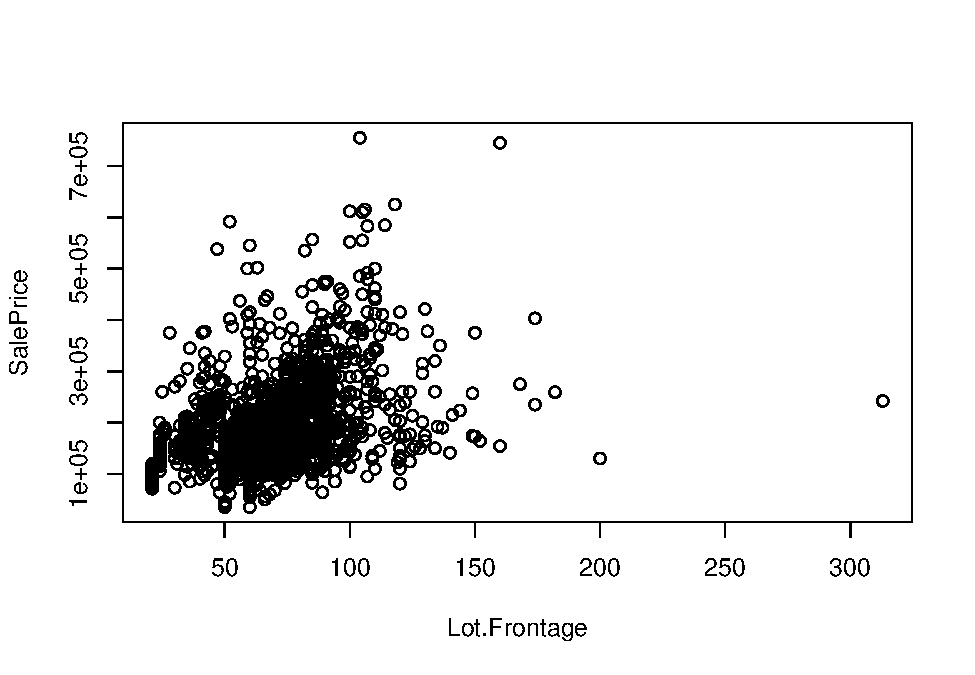
\includegraphics{Predicting-Housing-Price_files/figure-latex/unnamed-chunk-2-1.pdf}
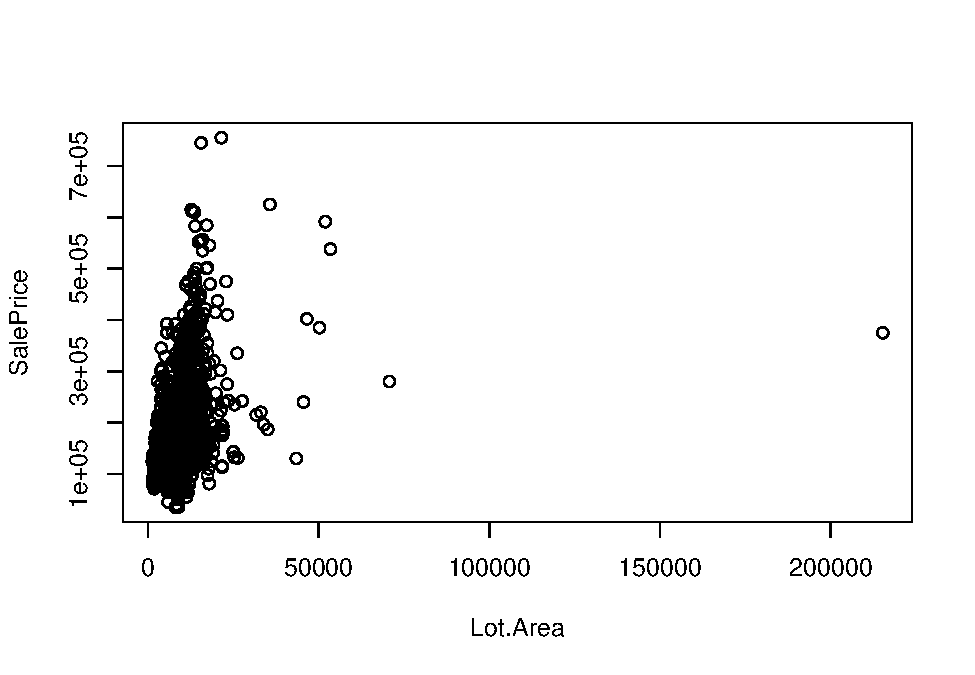
\includegraphics{Predicting-Housing-Price_files/figure-latex/unnamed-chunk-2-2.pdf}
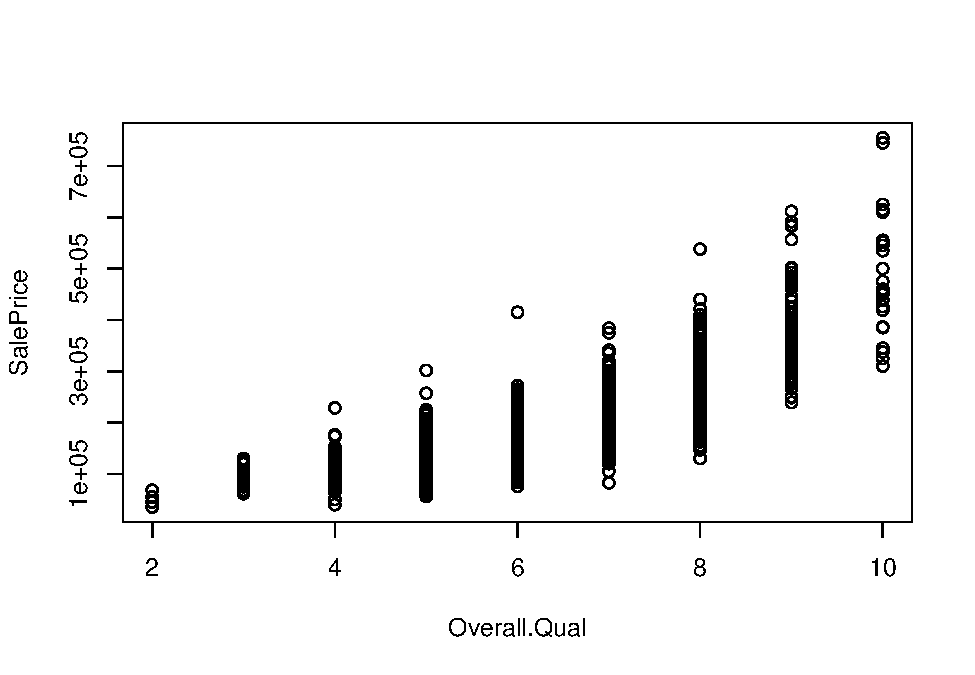
\includegraphics{Predicting-Housing-Price_files/figure-latex/unnamed-chunk-2-3.pdf}
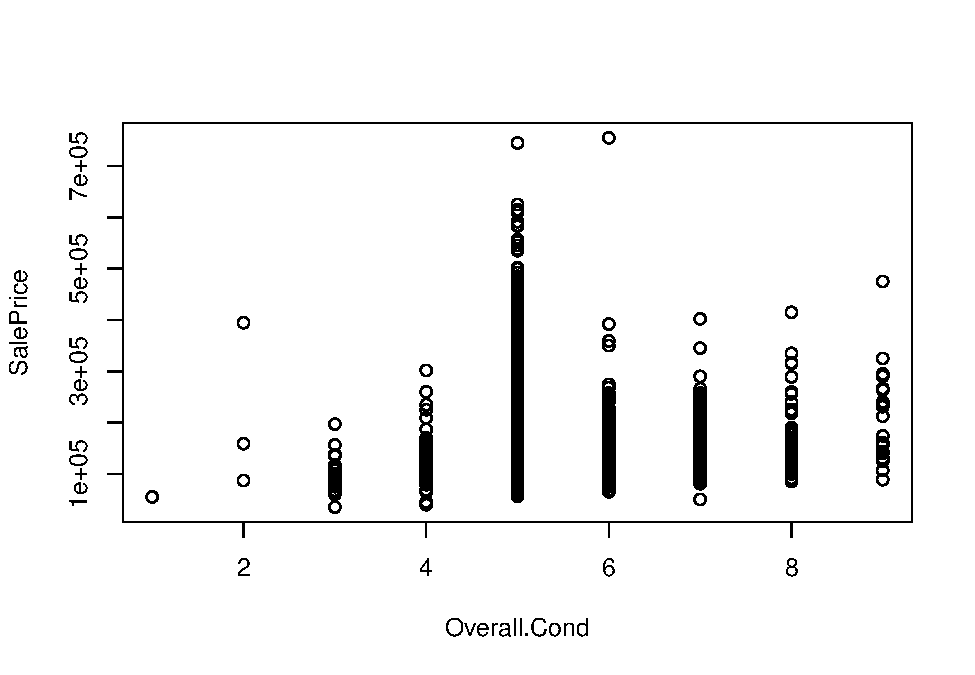
\includegraphics{Predicting-Housing-Price_files/figure-latex/unnamed-chunk-2-4.pdf}
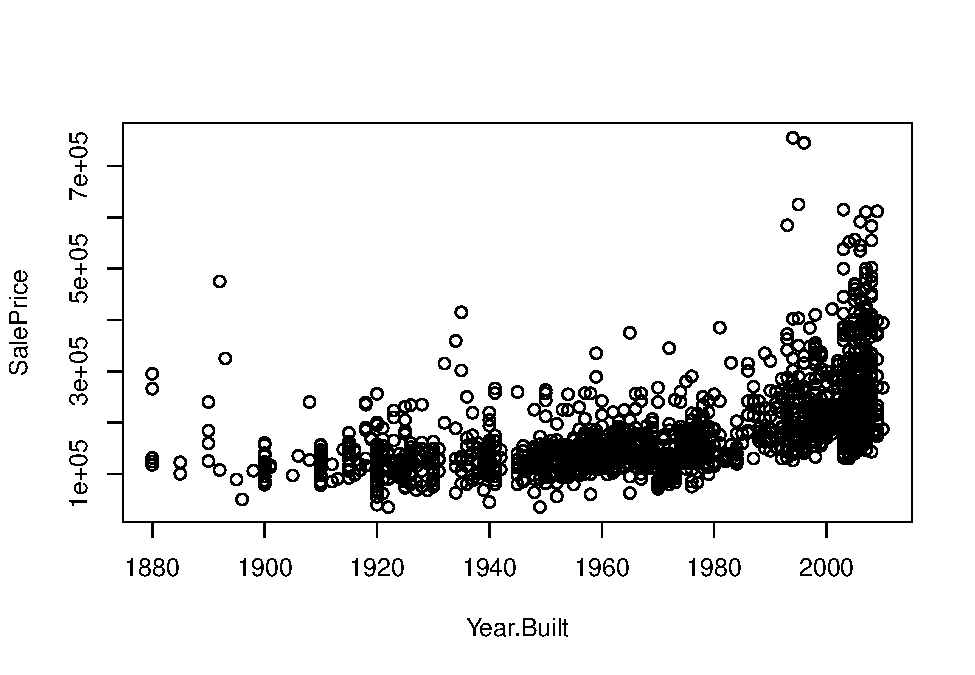
\includegraphics{Predicting-Housing-Price_files/figure-latex/unnamed-chunk-2-5.pdf}
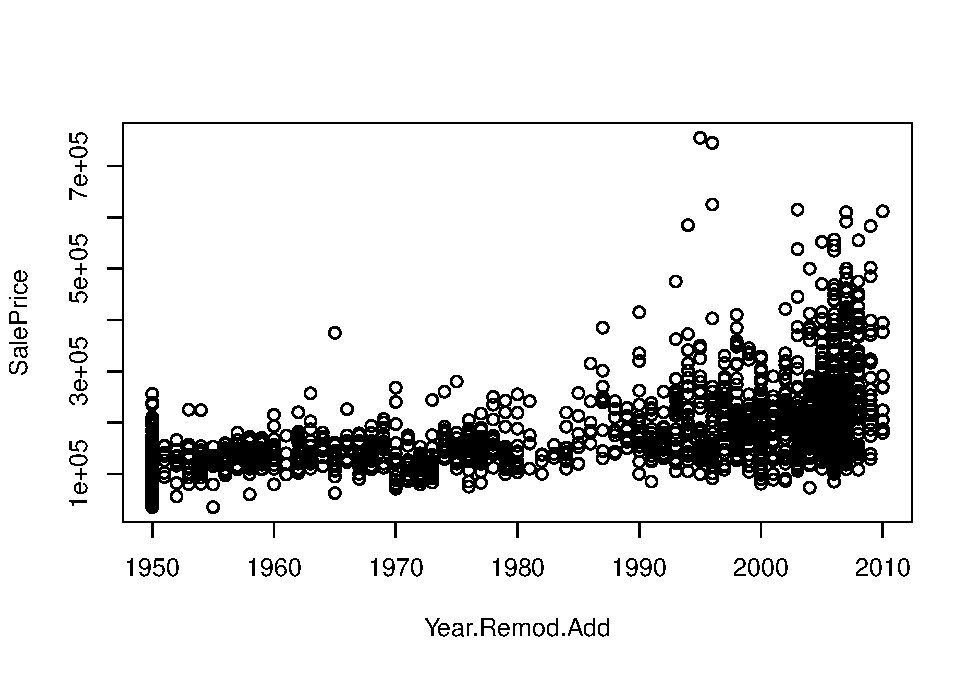
\includegraphics{Predicting-Housing-Price_files/figure-latex/unnamed-chunk-2-6.pdf}
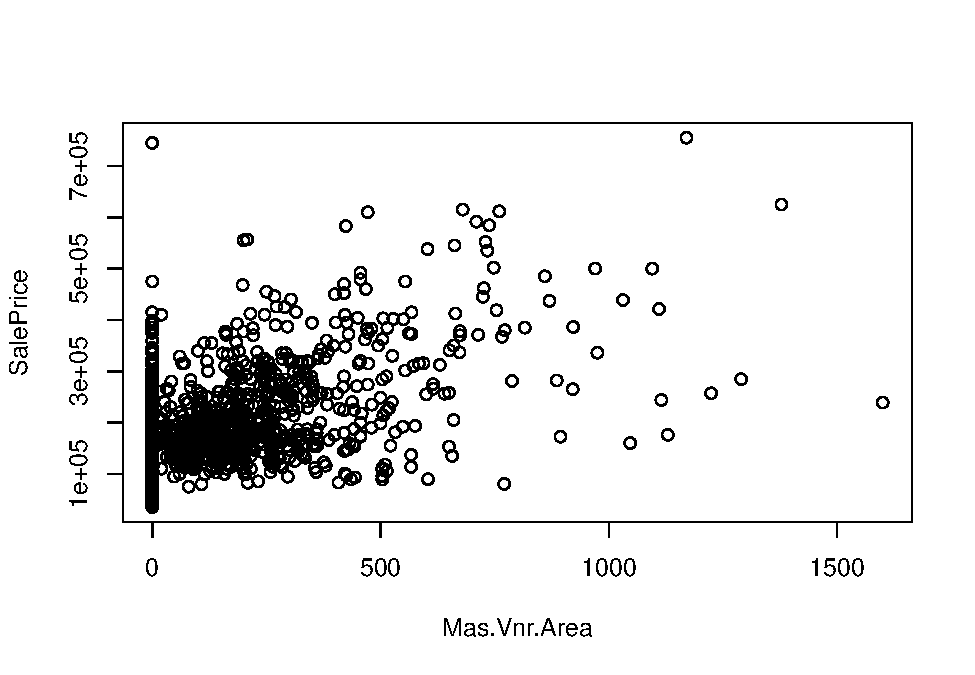
\includegraphics{Predicting-Housing-Price_files/figure-latex/unnamed-chunk-2-7.pdf}
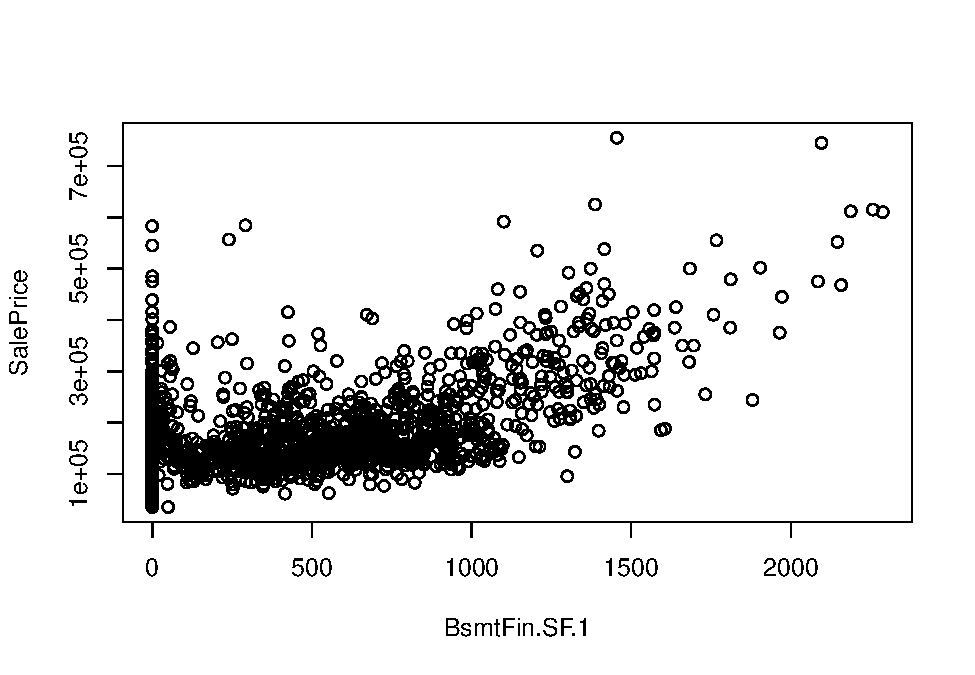
\includegraphics{Predicting-Housing-Price_files/figure-latex/unnamed-chunk-2-8.pdf}
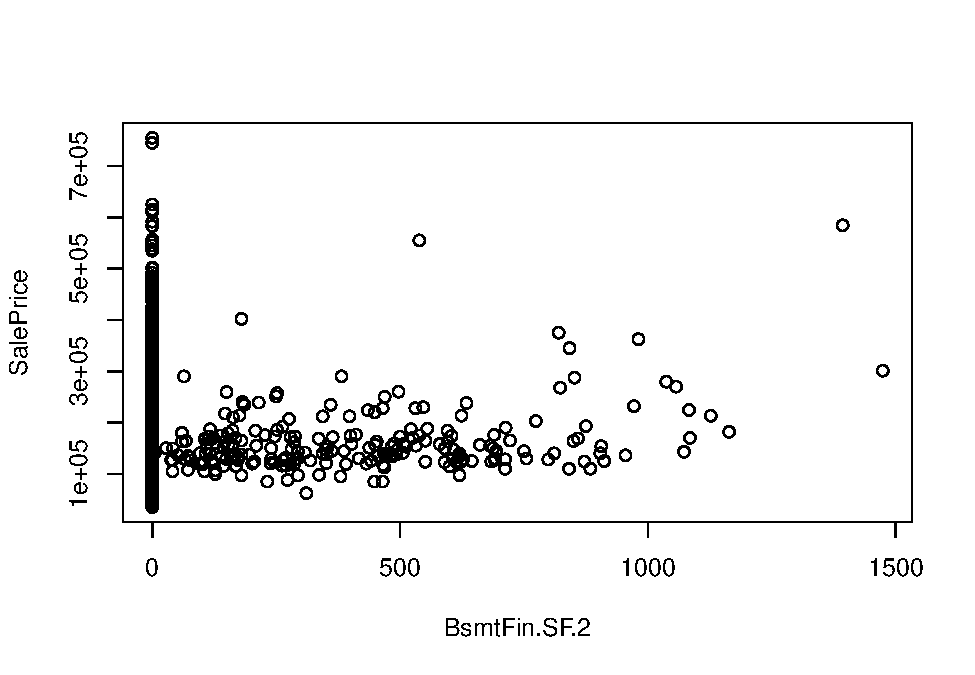
\includegraphics{Predicting-Housing-Price_files/figure-latex/unnamed-chunk-2-9.pdf}
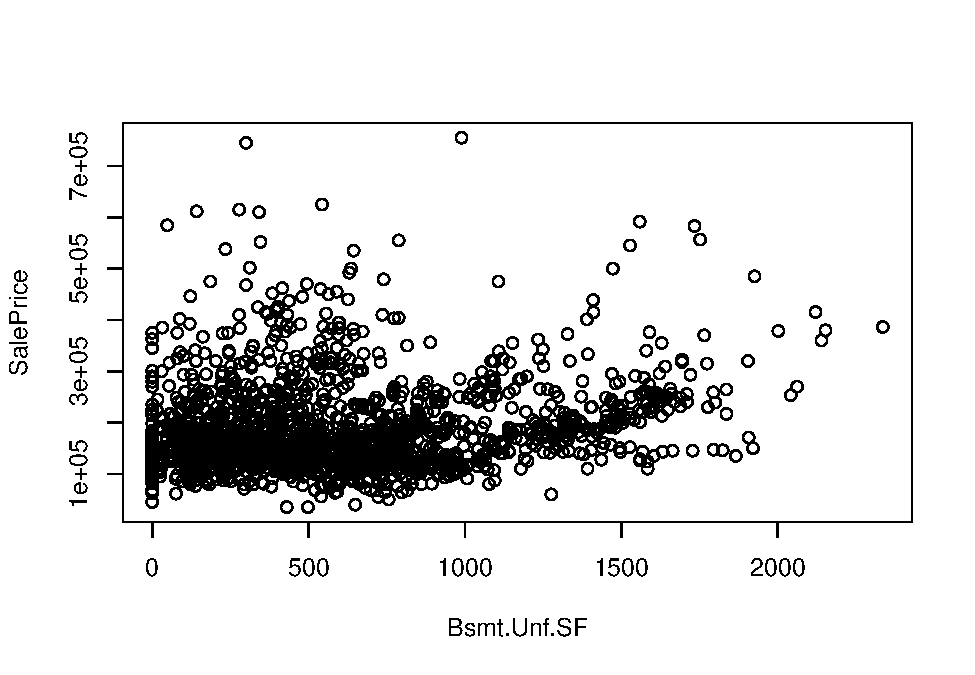
\includegraphics{Predicting-Housing-Price_files/figure-latex/unnamed-chunk-2-10.pdf}
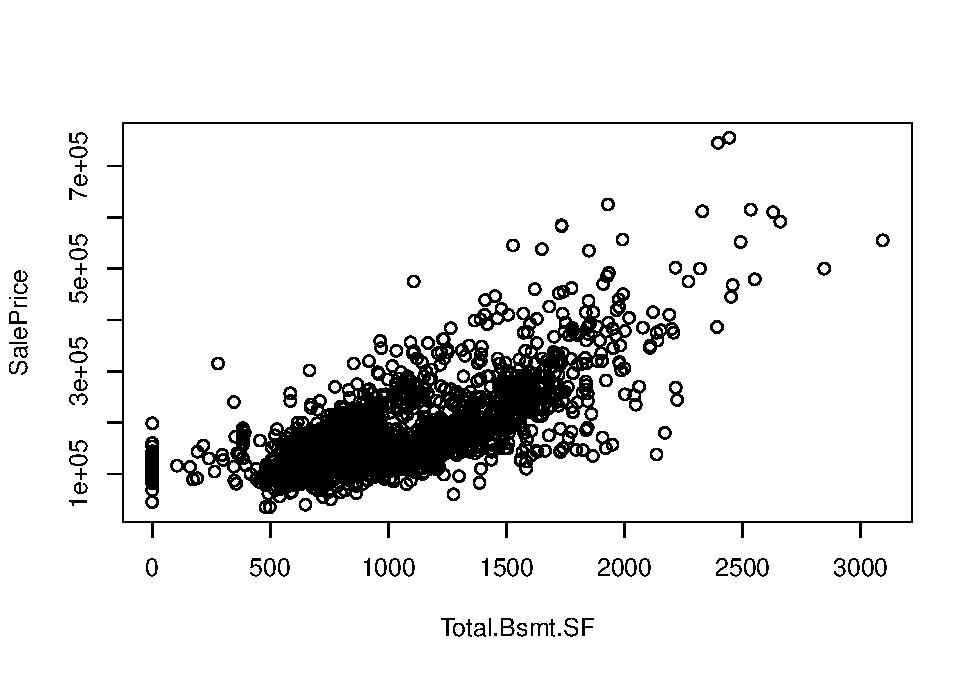
\includegraphics{Predicting-Housing-Price_files/figure-latex/unnamed-chunk-2-11.pdf}
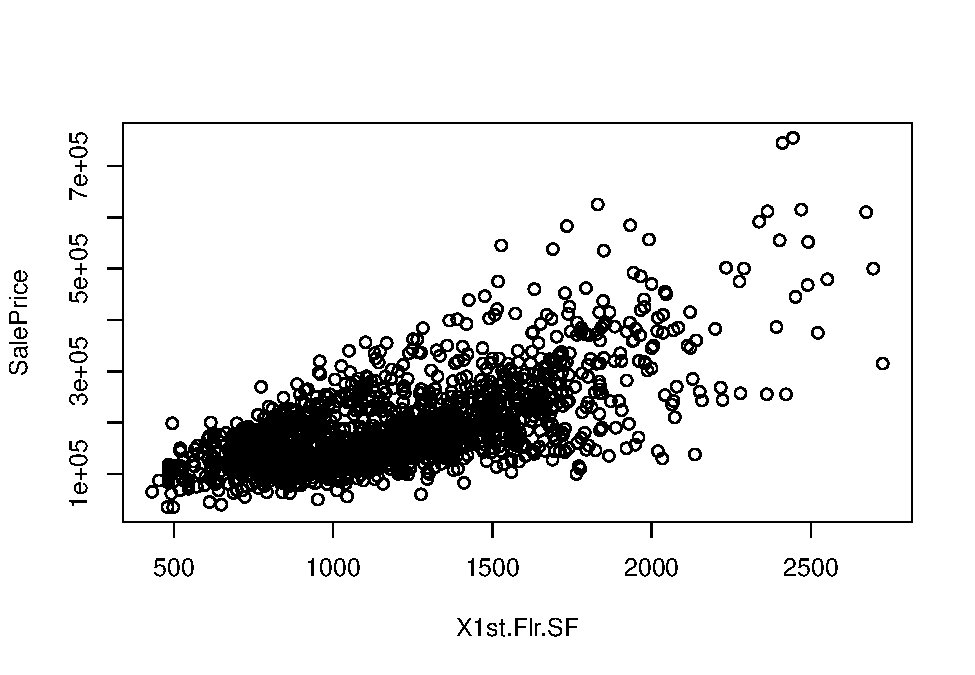
\includegraphics{Predicting-Housing-Price_files/figure-latex/unnamed-chunk-2-12.pdf}
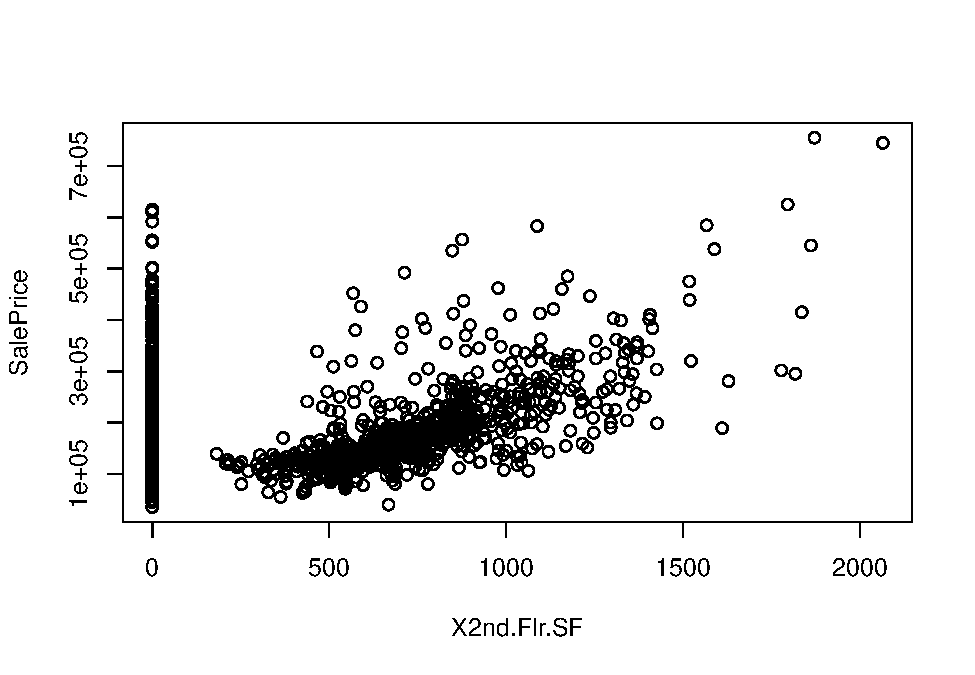
\includegraphics{Predicting-Housing-Price_files/figure-latex/unnamed-chunk-2-13.pdf}
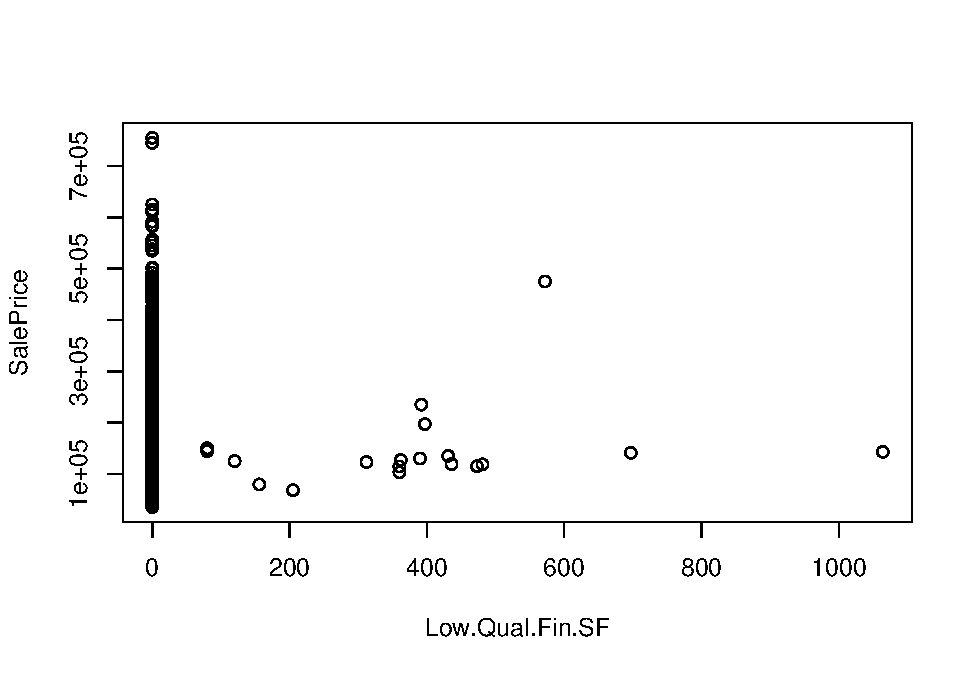
\includegraphics{Predicting-Housing-Price_files/figure-latex/unnamed-chunk-2-14.pdf}
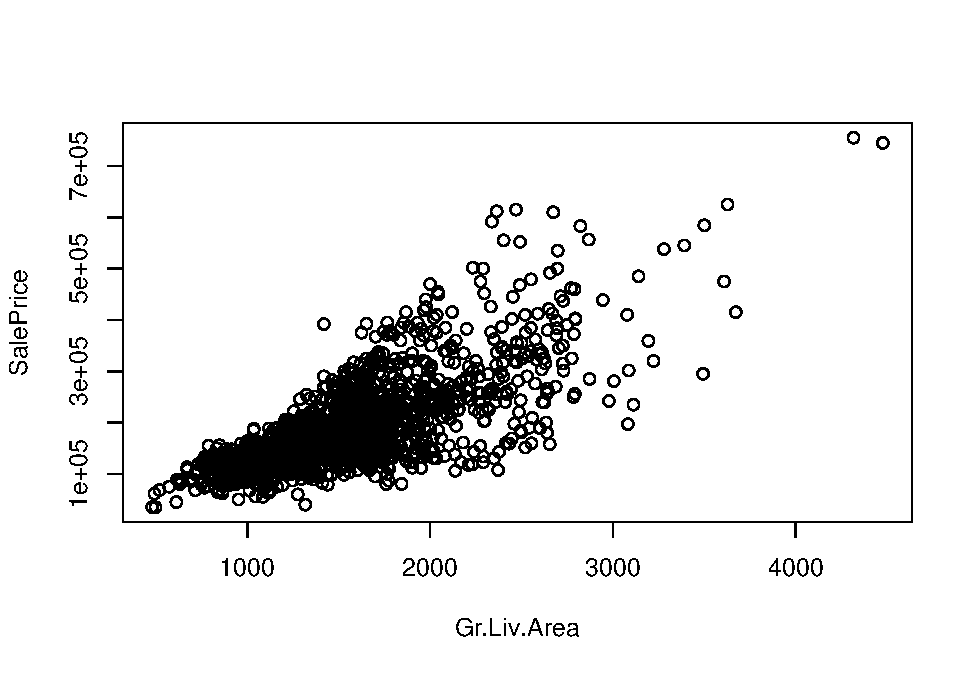
\includegraphics{Predicting-Housing-Price_files/figure-latex/unnamed-chunk-2-15.pdf}
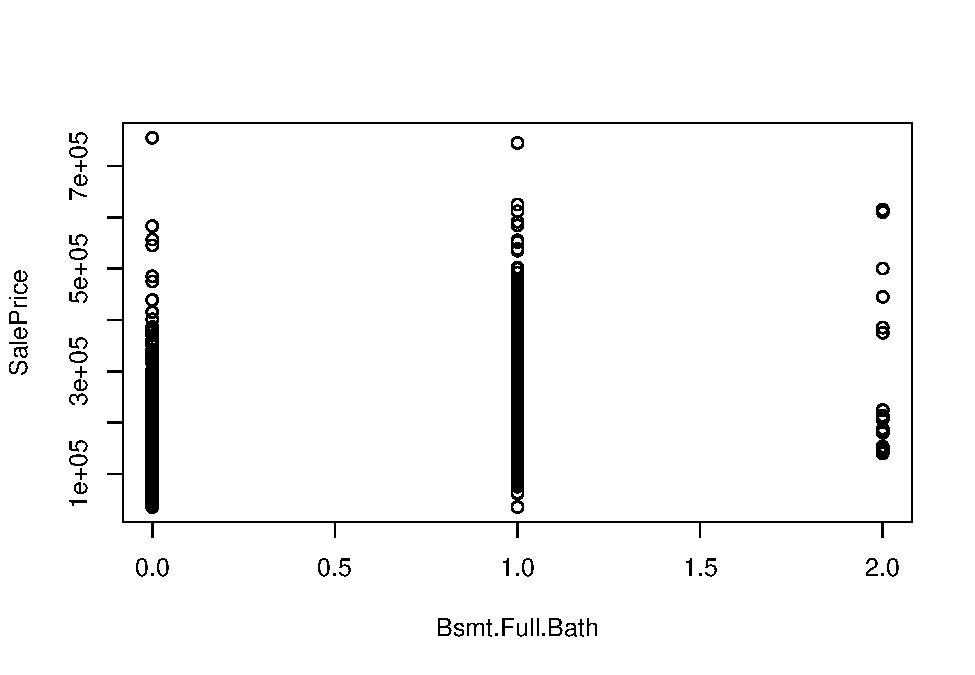
\includegraphics{Predicting-Housing-Price_files/figure-latex/unnamed-chunk-2-16.pdf}
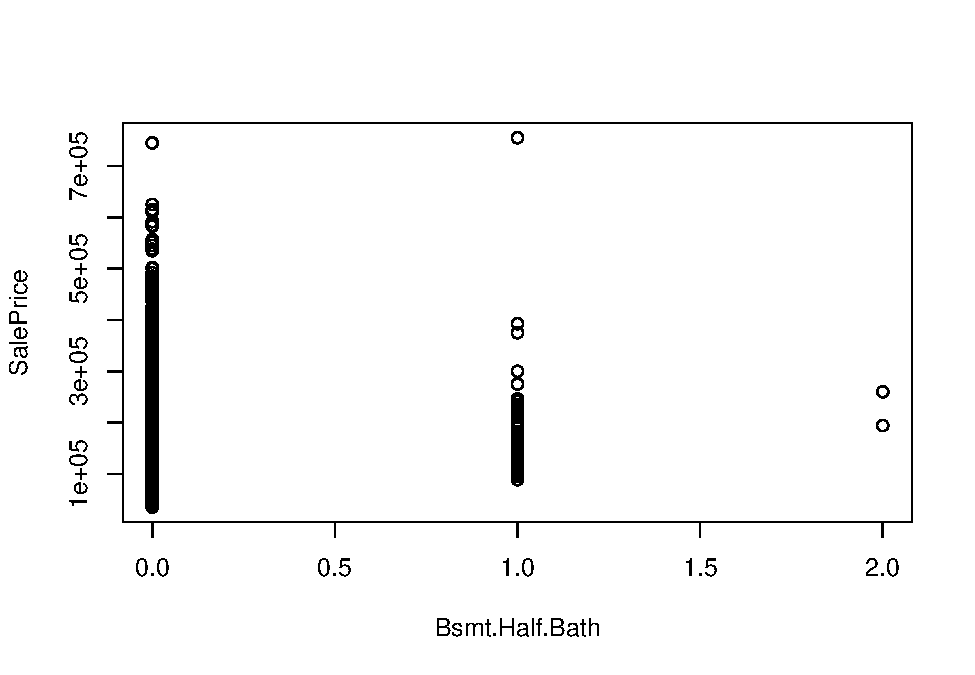
\includegraphics{Predicting-Housing-Price_files/figure-latex/unnamed-chunk-2-17.pdf}
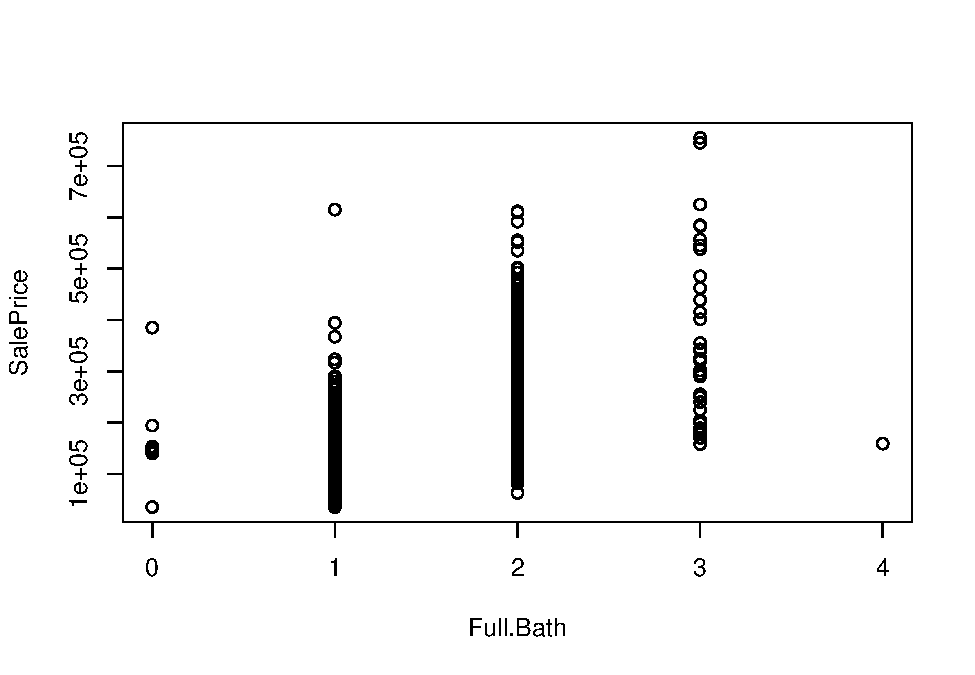
\includegraphics{Predicting-Housing-Price_files/figure-latex/unnamed-chunk-2-18.pdf}
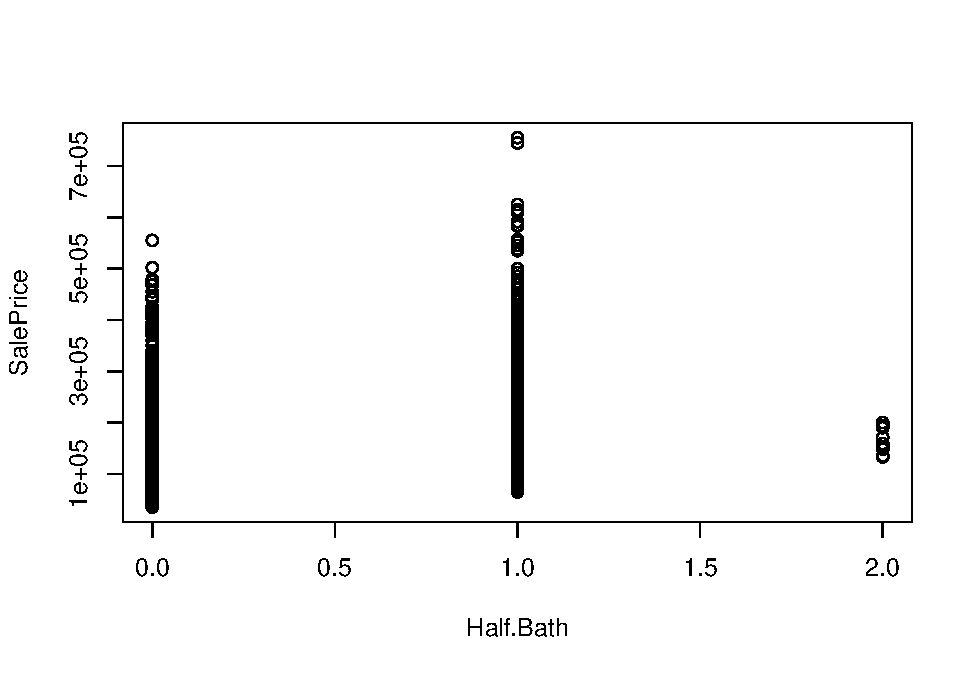
\includegraphics{Predicting-Housing-Price_files/figure-latex/unnamed-chunk-2-19.pdf}
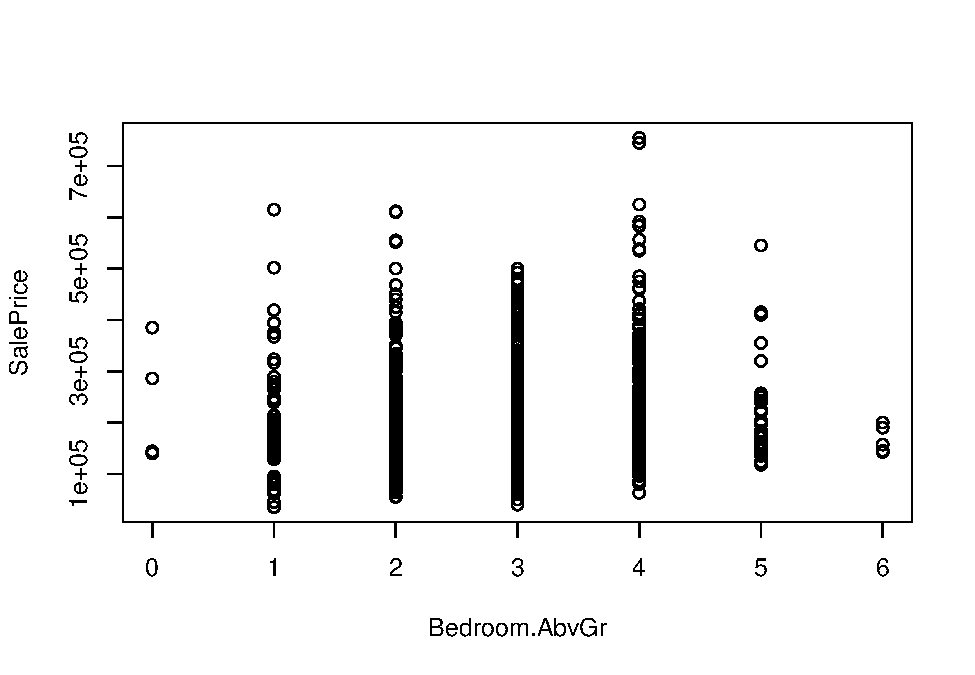
\includegraphics{Predicting-Housing-Price_files/figure-latex/unnamed-chunk-2-20.pdf}
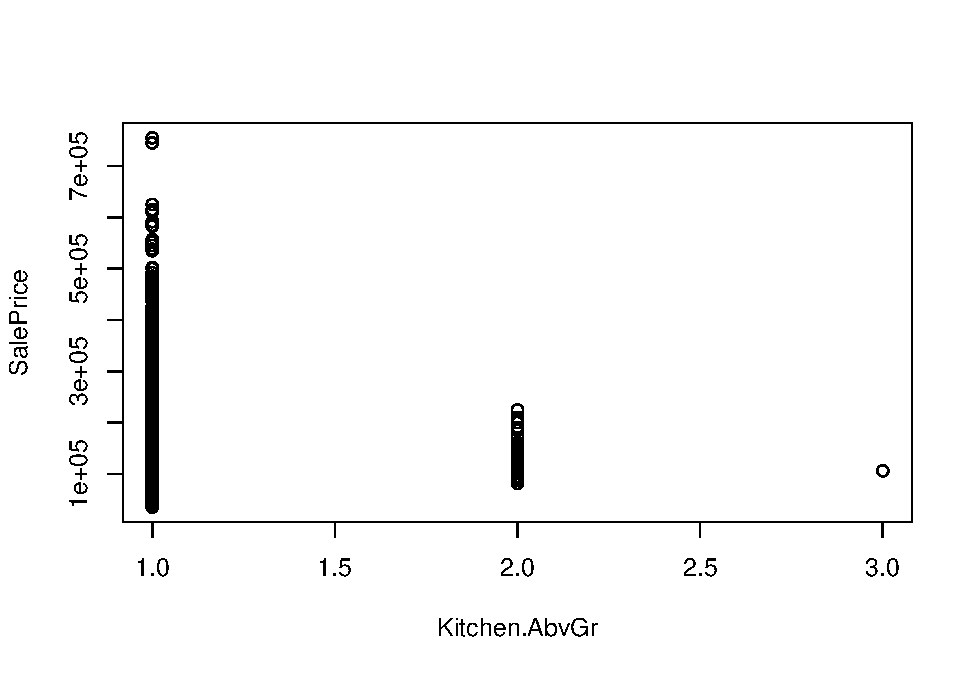
\includegraphics{Predicting-Housing-Price_files/figure-latex/unnamed-chunk-2-21.pdf}
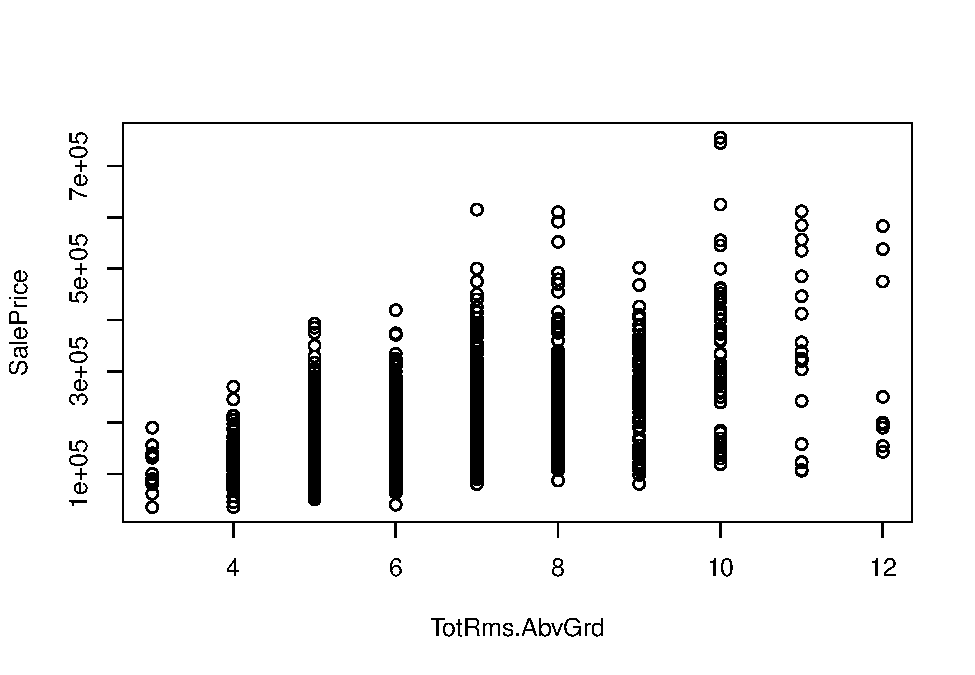
\includegraphics{Predicting-Housing-Price_files/figure-latex/unnamed-chunk-2-22.pdf}
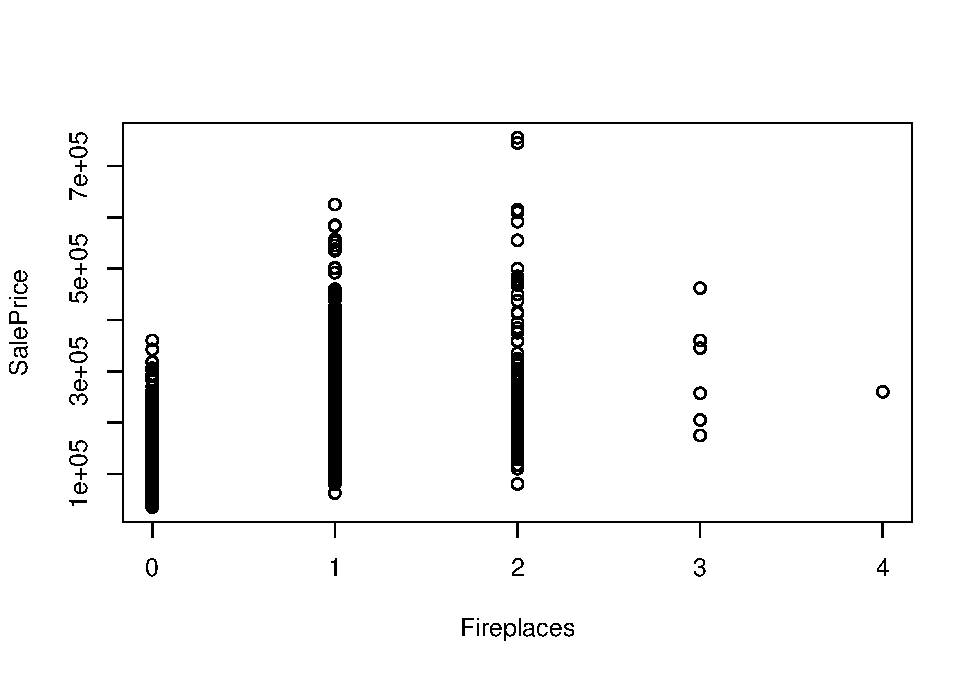
\includegraphics{Predicting-Housing-Price_files/figure-latex/unnamed-chunk-2-23.pdf}
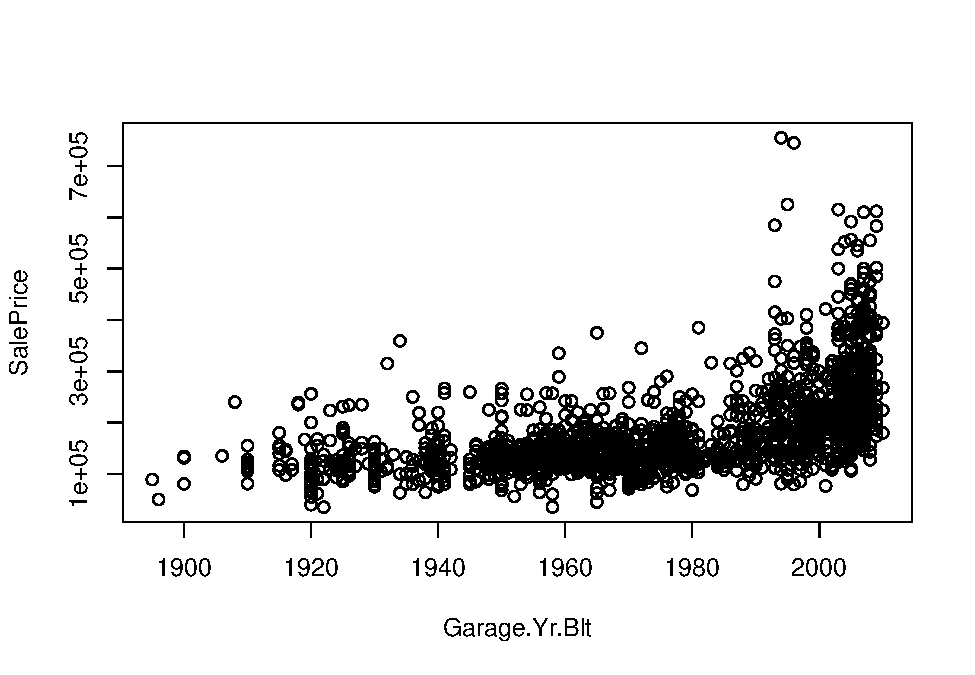
\includegraphics{Predicting-Housing-Price_files/figure-latex/unnamed-chunk-2-24.pdf}
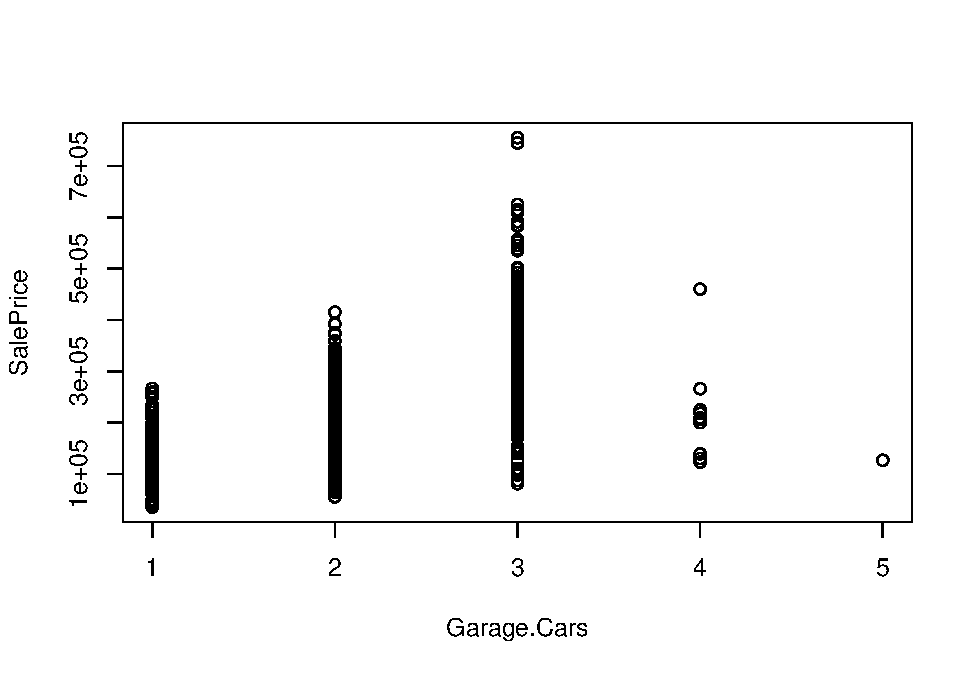
\includegraphics{Predicting-Housing-Price_files/figure-latex/unnamed-chunk-2-25.pdf}
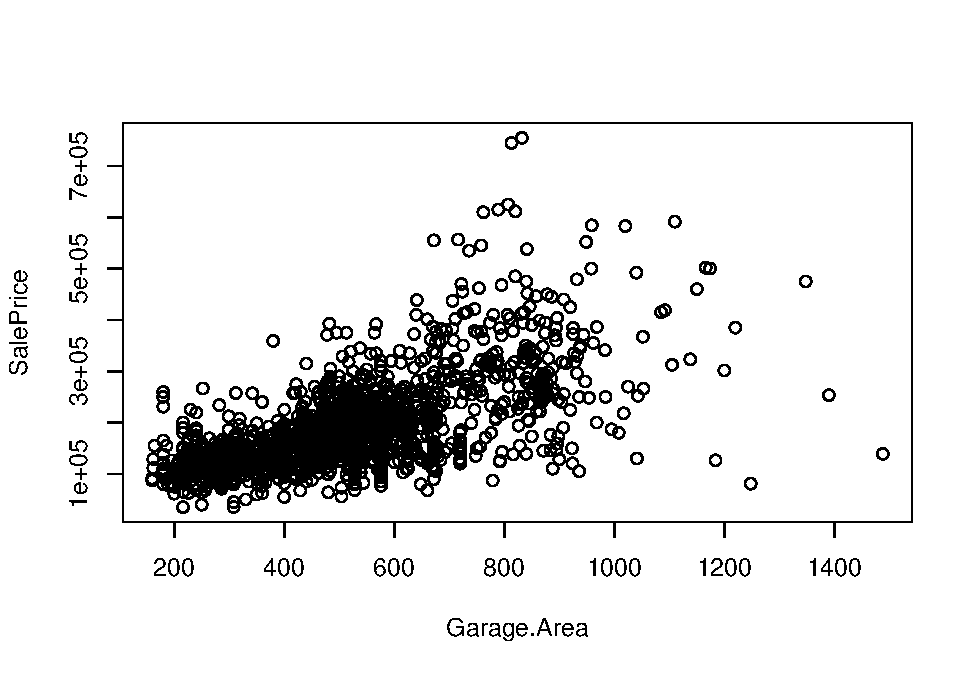
\includegraphics{Predicting-Housing-Price_files/figure-latex/unnamed-chunk-2-26.pdf}
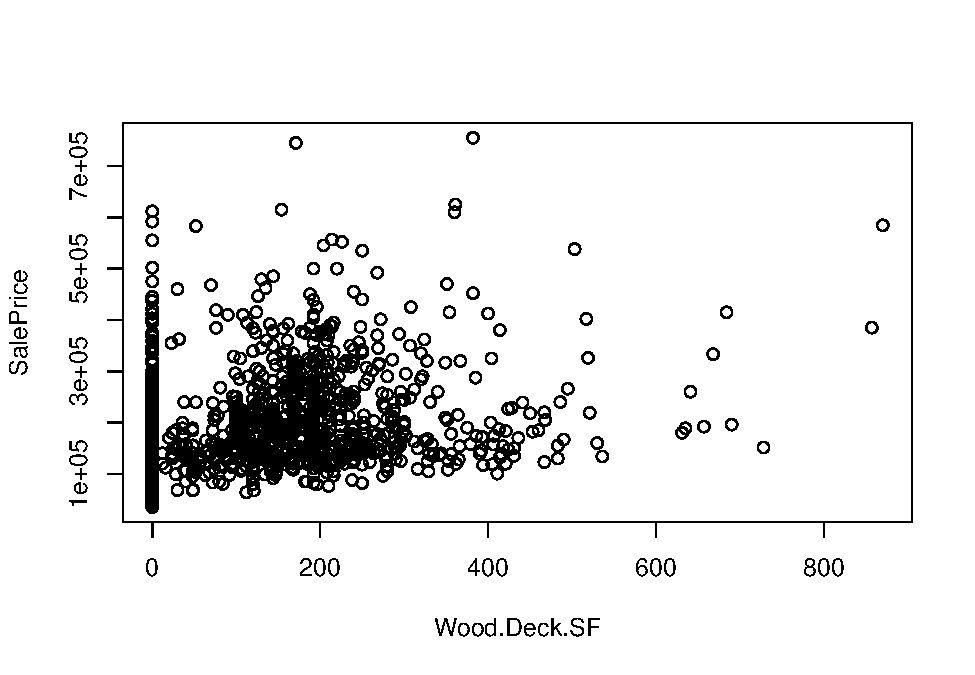
\includegraphics{Predicting-Housing-Price_files/figure-latex/unnamed-chunk-2-27.pdf}
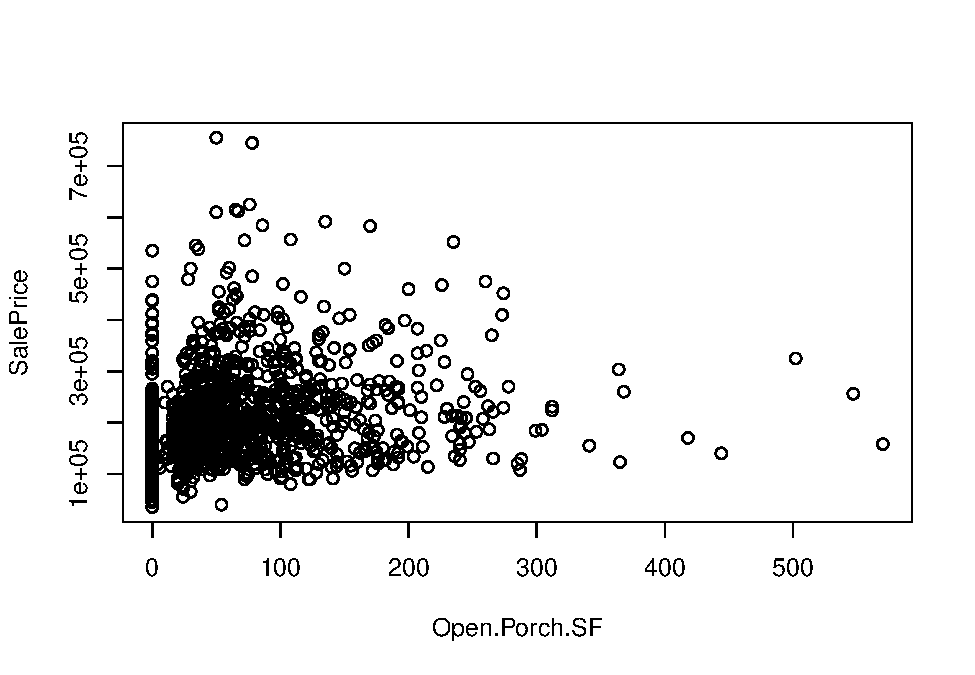
\includegraphics{Predicting-Housing-Price_files/figure-latex/unnamed-chunk-2-28.pdf}
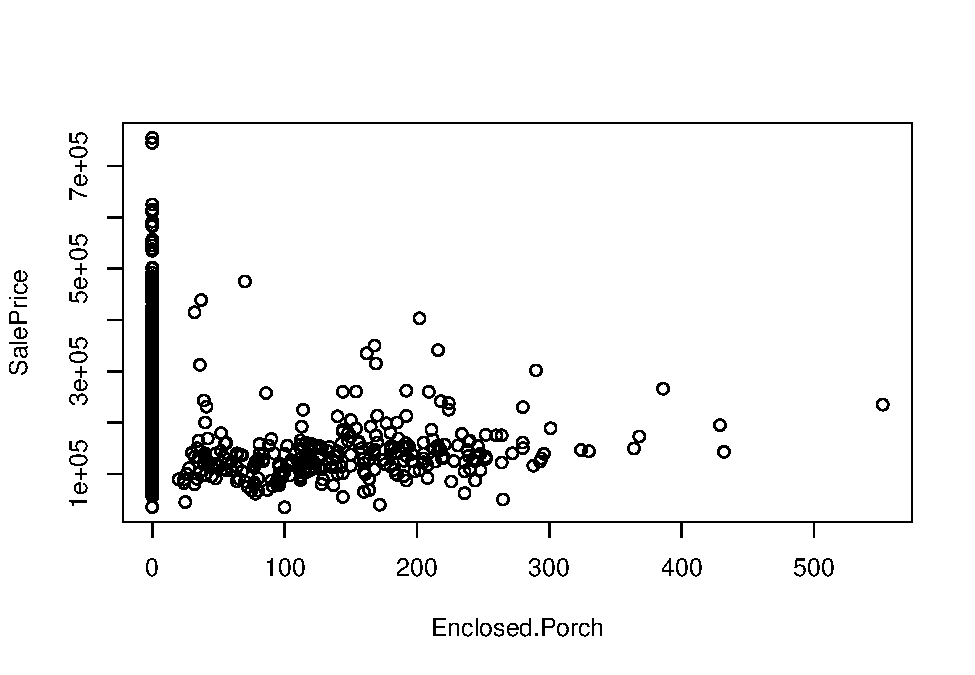
\includegraphics{Predicting-Housing-Price_files/figure-latex/unnamed-chunk-2-29.pdf}
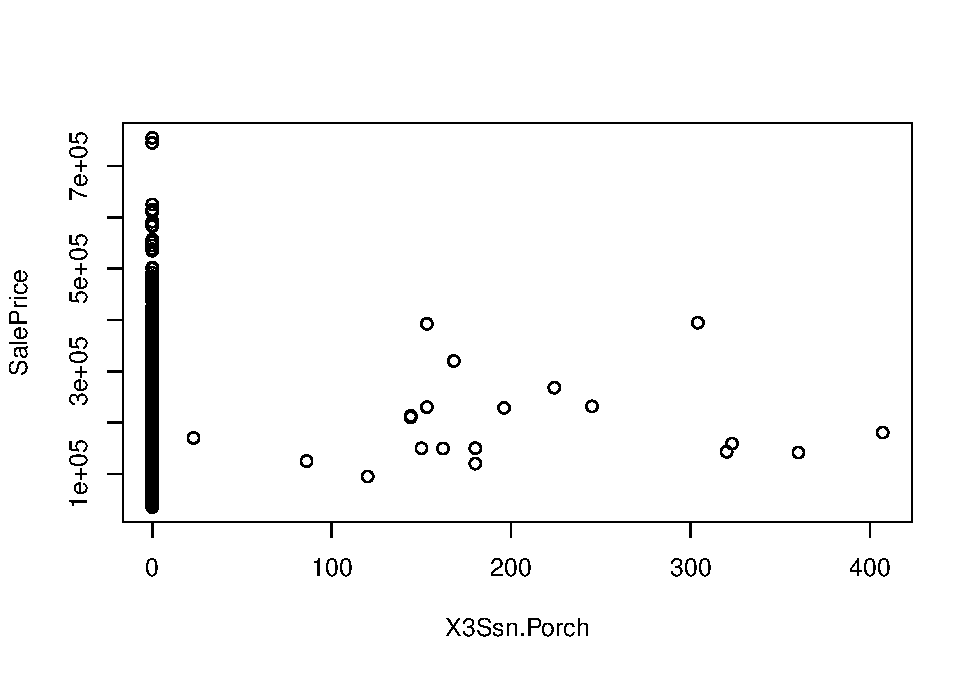
\includegraphics{Predicting-Housing-Price_files/figure-latex/unnamed-chunk-2-30.pdf}
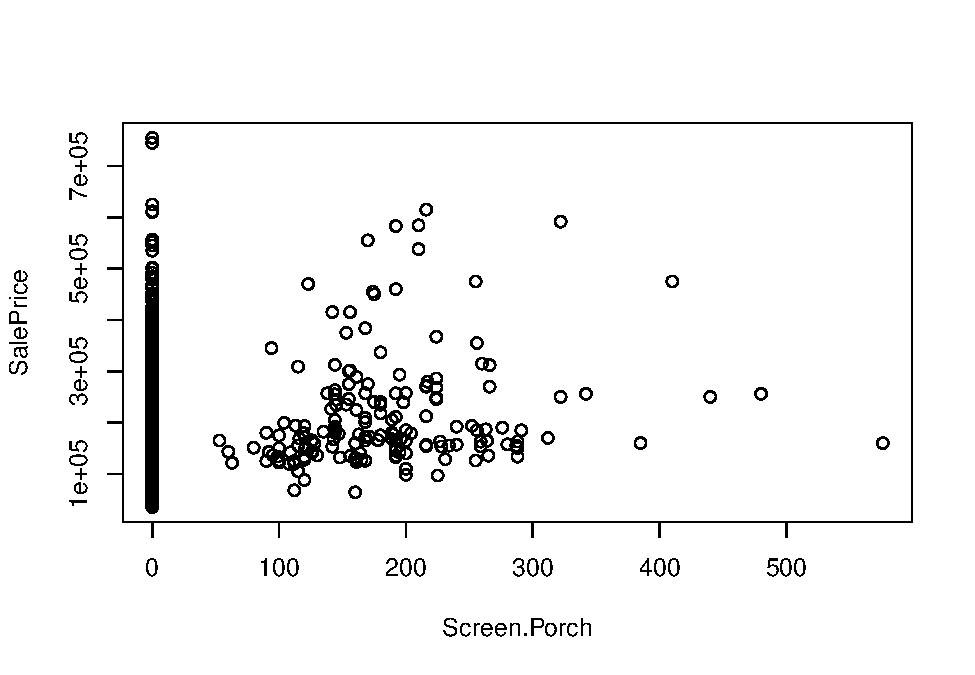
\includegraphics{Predicting-Housing-Price_files/figure-latex/unnamed-chunk-2-31.pdf}
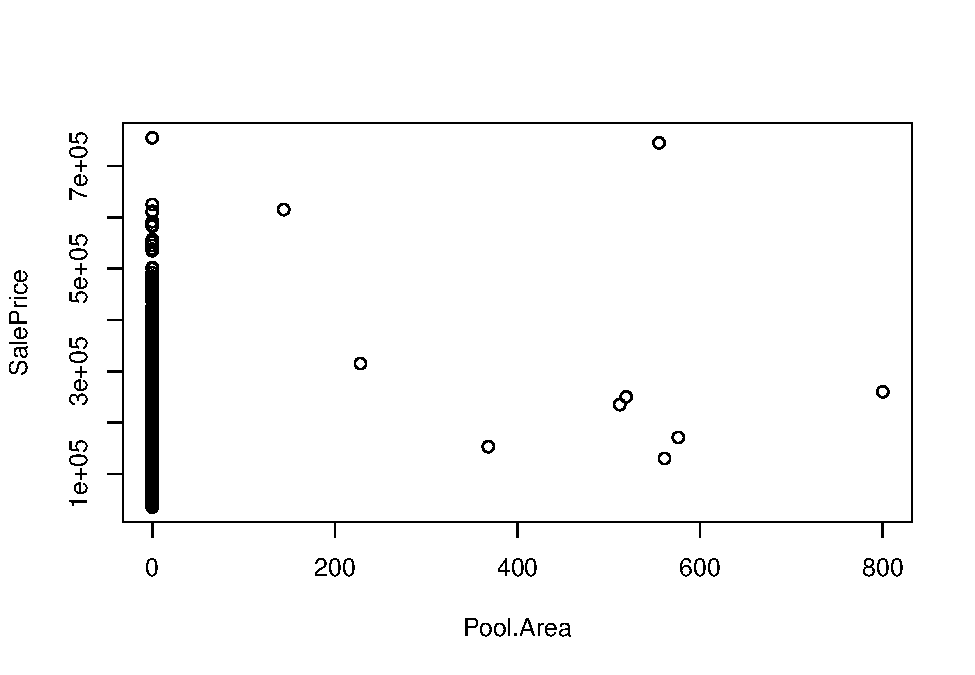
\includegraphics{Predicting-Housing-Price_files/figure-latex/unnamed-chunk-2-32.pdf}
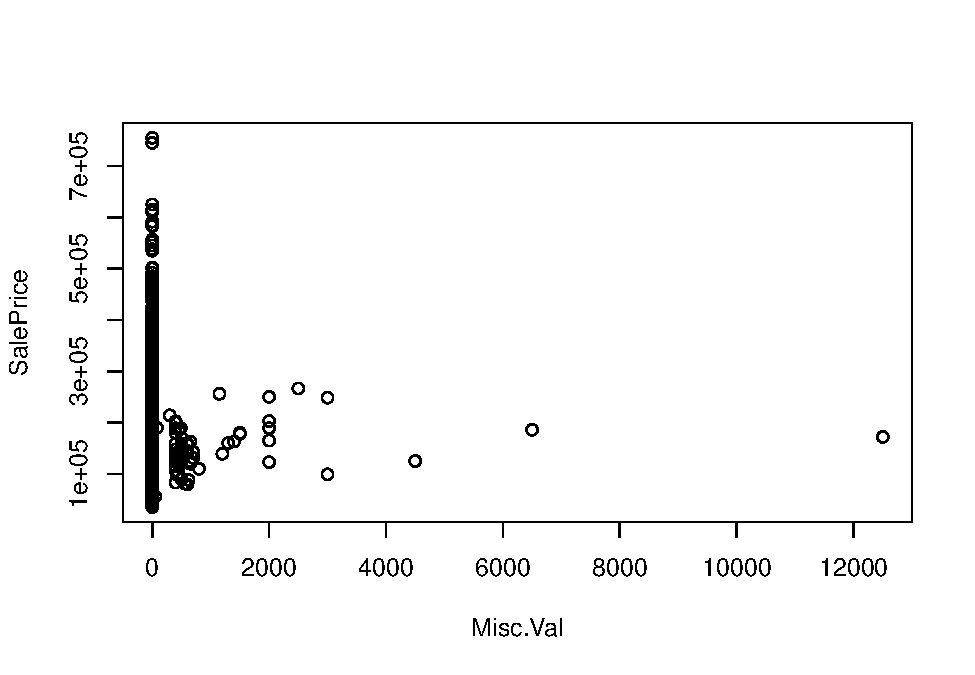
\includegraphics{Predicting-Housing-Price_files/figure-latex/unnamed-chunk-2-33.pdf}
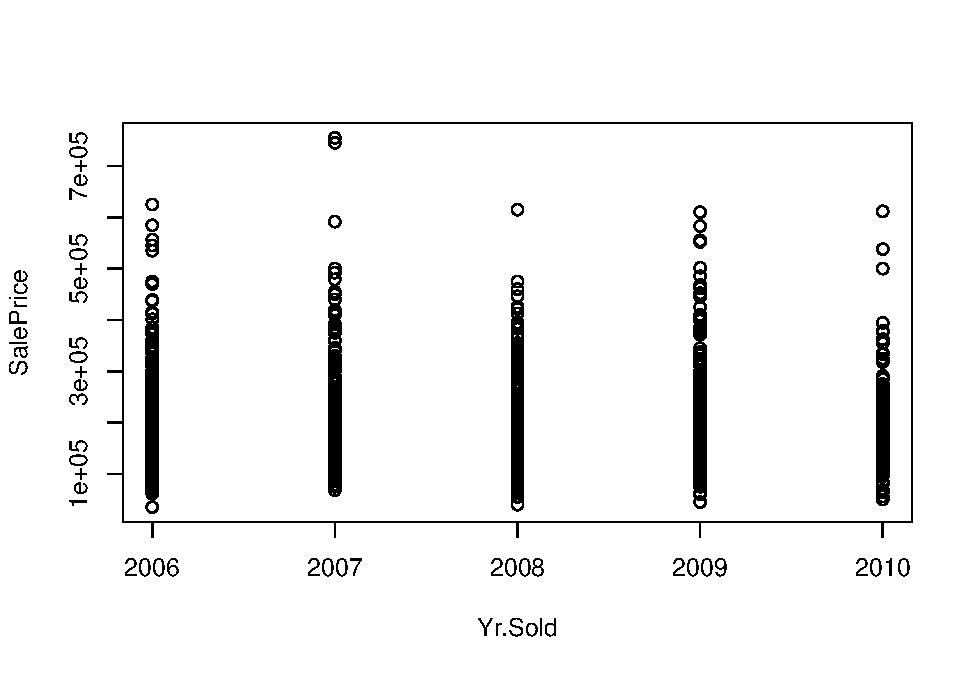
\includegraphics{Predicting-Housing-Price_files/figure-latex/unnamed-chunk-2-34.pdf}
\# Modeling:

\begin{Shaded}
\begin{Highlighting}[]
\CommentTok{# Create First Model:}
\NormalTok{fit <-}\StringTok{ }\KeywordTok{lm}\NormalTok{(SalePrice }\OperatorTok{~}\StringTok{ }\NormalTok{Overall.Qual }\OperatorTok{+}\StringTok{ }\NormalTok{Year.Built }\OperatorTok{+}\StringTok{ }\NormalTok{Year.Remod.Add }\OperatorTok{+}\StringTok{ }\NormalTok{BsmtFin.SF}\FloatTok{.1} \OperatorTok{+}\StringTok{ }\NormalTok{Total.Bsmt.SF }\OperatorTok{+}\StringTok{ }\NormalTok{X1st.Flr.SF }\OperatorTok{+}\StringTok{ }\NormalTok{Gr.Liv.Area }\OperatorTok{+}\StringTok{ }\NormalTok{TotRms.AbvGrd }\OperatorTok{+}
\StringTok{            }\NormalTok{Garage.Yr.Blt }\OperatorTok{+}\StringTok{ }\NormalTok{Wood.Deck.SF }\OperatorTok{+}\StringTok{  }\NormalTok{Open.Porch.SF, }\DataTypeTok{data =}\NormalTok{ num.ames, }\DataTypeTok{subset =}\NormalTok{ train)}

\CommentTok{# Return model summary of first model:}
\KeywordTok{summary}\NormalTok{(fit)}
\end{Highlighting}
\end{Shaded}

\begin{verbatim}
## 
## Call:
## lm(formula = SalePrice ~ Overall.Qual + Year.Built + Year.Remod.Add + 
##     BsmtFin.SF.1 + Total.Bsmt.SF + X1st.Flr.SF + Gr.Liv.Area + 
##     TotRms.AbvGrd + Garage.Yr.Blt + Wood.Deck.SF + Open.Porch.SF, 
##     data = num.ames, subset = train)
## 
## Residuals:
##     Min      1Q  Median      3Q     Max 
## -136957  -18417   -1373   16771  230613 
## 
## Coefficients:
##                  Estimate Std. Error t value Pr(>|t|)    
## (Intercept)    -1.119e+06  9.574e+04 -11.689  < 2e-16 ***
## Overall.Qual    1.966e+04  9.020e+02  21.791  < 2e-16 ***
## Year.Built      1.537e+02  4.895e+01   3.141 0.001714 ** 
## Year.Remod.Add  2.550e+02  5.246e+01   4.860 1.27e-06 ***
## BsmtFin.SF.1    3.251e+01  2.062e+00  15.767  < 2e-16 ***
## Total.Bsmt.SF   2.694e+01  3.472e+00   7.759 1.43e-14 ***
## X1st.Flr.SF     1.274e+01  3.754e+00   3.393 0.000706 ***
## Gr.Liv.Area     6.844e+01  3.282e+00  20.853  < 2e-16 ***
## TotRms.AbvGrd  -1.002e+03  8.885e+02  -1.128 0.259577    
## Garage.Yr.Blt   1.097e+02  5.597e+01   1.960 0.050202 .  
## Wood.Deck.SF    1.843e+01  6.779e+00   2.718 0.006621 ** 
## Open.Porch.SF   1.395e+01  1.291e+01   1.080 0.280151    
## ---
## Signif. codes:  0 '***' 0.001 '**' 0.01 '*' 0.05 '.' 0.1 ' ' 1
## 
## Residual standard error: 32820 on 1788 degrees of freedom
## Multiple R-squared:  0.8528, Adjusted R-squared:  0.8519 
## F-statistic: 941.6 on 11 and 1788 DF,  p-value: < 2.2e-16
\end{verbatim}

\begin{Shaded}
\begin{Highlighting}[]
\CommentTok{# Create Second Model:}
\NormalTok{fit2 <-}\StringTok{ }\KeywordTok{lm}\NormalTok{(SalePrice }\OperatorTok{~}\StringTok{ }\NormalTok{Overall.Qual }\OperatorTok{+}\StringTok{ }\NormalTok{Year.Built }\OperatorTok{+}\StringTok{ }\NormalTok{Year.Remod.Add }\OperatorTok{+}\StringTok{ }\NormalTok{BsmtFin.SF}\FloatTok{.1} \OperatorTok{+}\StringTok{ }\NormalTok{Total.Bsmt.SF }\OperatorTok{+}\StringTok{ }\NormalTok{X1st.Flr.SF }\OperatorTok{+}\StringTok{ }\NormalTok{Gr.Liv.Area }\OperatorTok{+}\StringTok{ }\NormalTok{TotRms.AbvGrd }\OperatorTok{+}
\StringTok{            }\NormalTok{Garage.Yr.Blt }\OperatorTok{+}\StringTok{ }\NormalTok{Wood.Deck.SF, }\DataTypeTok{data =}\NormalTok{ num.ames, }\DataTypeTok{subset =}\NormalTok{ train)}
\CommentTok{# Return model summary of second model:}
\KeywordTok{summary}\NormalTok{(fit2)}
\end{Highlighting}
\end{Shaded}

\begin{verbatim}
## 
## Call:
## lm(formula = SalePrice ~ Overall.Qual + Year.Built + Year.Remod.Add + 
##     BsmtFin.SF.1 + Total.Bsmt.SF + X1st.Flr.SF + Gr.Liv.Area + 
##     TotRms.AbvGrd + Garage.Yr.Blt + Wood.Deck.SF, data = num.ames, 
##     subset = train)
## 
## Residuals:
##     Min      1Q  Median      3Q     Max 
## -137514  -18485   -1627   16894  231403 
## 
## Coefficients:
##                  Estimate Std. Error t value Pr(>|t|)    
## (Intercept)    -1.136e+06  9.446e+04 -12.026  < 2e-16 ***
## Overall.Qual    1.966e+04  9.020e+02  21.796  < 2e-16 ***
## Year.Built      1.542e+02  4.895e+01   3.151 0.001656 ** 
## Year.Remod.Add  2.605e+02  5.221e+01   4.991 6.60e-07 ***
## BsmtFin.SF.1    3.251e+01  2.062e+00  15.765  < 2e-16 ***
## Total.Bsmt.SF   2.723e+01  3.462e+00   7.866 6.26e-15 ***
## X1st.Flr.SF     1.256e+01  3.750e+00   3.349 0.000827 ***
## Gr.Liv.Area     6.900e+01  3.241e+00  21.292  < 2e-16 ***
## TotRms.AbvGrd  -1.034e+03  8.881e+02  -1.164 0.244550    
## Garage.Yr.Blt   1.121e+02  5.593e+01   2.004 0.045181 *  
## Wood.Deck.SF    1.775e+01  6.750e+00   2.630 0.008619 ** 
## ---
## Signif. codes:  0 '***' 0.001 '**' 0.01 '*' 0.05 '.' 0.1 ' ' 1
## 
## Residual standard error: 32820 on 1789 degrees of freedom
## Multiple R-squared:  0.8527, Adjusted R-squared:  0.8519 
## F-statistic:  1036 on 10 and 1789 DF,  p-value: < 2.2e-16
\end{verbatim}

\begin{Shaded}
\begin{Highlighting}[]
\CommentTok{# Create Third Model:}
\NormalTok{fit3 <-}\StringTok{ }\KeywordTok{lm}\NormalTok{(SalePrice }\OperatorTok{~}\StringTok{ }\NormalTok{Overall.Qual }\OperatorTok{+}\StringTok{ }\NormalTok{Year.Built }\OperatorTok{+}\StringTok{ }\NormalTok{Year.Remod.Add }\OperatorTok{+}\StringTok{ }\NormalTok{BsmtFin.SF}\FloatTok{.1} \OperatorTok{+}\StringTok{ }\NormalTok{Total.Bsmt.SF }\OperatorTok{+}\StringTok{ }\NormalTok{X1st.Flr.SF }\OperatorTok{+}\StringTok{ }\NormalTok{Gr.Liv.Area }\OperatorTok{+}\StringTok{ }\NormalTok{Garage.Yr.Blt }\OperatorTok{+}\StringTok{ }\NormalTok{Wood.Deck.SF, }\DataTypeTok{data =}\NormalTok{ num.ames, }\DataTypeTok{subset =}\NormalTok{ train)}
\CommentTok{# Return model summary of third model:}
\KeywordTok{summary}\NormalTok{(fit3)}
\end{Highlighting}
\end{Shaded}

\begin{verbatim}
## 
## Call:
## lm(formula = SalePrice ~ Overall.Qual + Year.Built + Year.Remod.Add + 
##     BsmtFin.SF.1 + Total.Bsmt.SF + X1st.Flr.SF + Gr.Liv.Area + 
##     Garage.Yr.Blt + Wood.Deck.SF, data = num.ames, subset = train)
## 
## Residuals:
##     Min      1Q  Median      3Q     Max 
## -137509  -18564   -1665   17169  229284 
## 
## Coefficients:
##                  Estimate Std. Error t value Pr(>|t|)    
## (Intercept)    -1.140e+06  9.442e+04 -12.070  < 2e-16 ***
## Overall.Qual    1.974e+04  8.993e+02  21.955  < 2e-16 ***
## Year.Built      1.534e+02  4.895e+01   3.134 0.001749 ** 
## Year.Remod.Add  2.620e+02  5.220e+01   5.020 5.67e-07 ***
## BsmtFin.SF.1    3.285e+01  2.041e+00  16.091  < 2e-16 ***
## Total.Bsmt.SF   2.725e+01  3.462e+00   7.872 5.99e-15 ***
## X1st.Flr.SF     1.258e+01  3.751e+00   3.353 0.000816 ***
## Gr.Liv.Area     6.619e+01  2.160e+00  30.642  < 2e-16 ***
## Garage.Yr.Blt   1.116e+02  5.593e+01   1.995 0.046140 *  
## Wood.Deck.SF    1.787e+01  6.750e+00   2.648 0.008169 ** 
## ---
## Signif. codes:  0 '***' 0.001 '**' 0.01 '*' 0.05 '.' 0.1 ' ' 1
## 
## Residual standard error: 32830 on 1790 degrees of freedom
## Multiple R-squared:  0.8526, Adjusted R-squared:  0.8518 
## F-statistic:  1150 on 9 and 1790 DF,  p-value: < 2.2e-16
\end{verbatim}

\hypertarget{check-model-diagnostics}{%
\section{Check Model Diagnostics:}\label{check-model-diagnostics}}

\begin{Shaded}
\begin{Highlighting}[]
\CommentTok{# Plot Fitted vs Residuals:}
\KeywordTok{plot}\NormalTok{(fit3}\OperatorTok{$}\NormalTok{res}\OperatorTok{~}\NormalTok{fit3}\OperatorTok{$}\NormalTok{fitted, }\DataTypeTok{main =} \StringTok{"Fitted vs Residuals"}\NormalTok{)}
\end{Highlighting}
\end{Shaded}

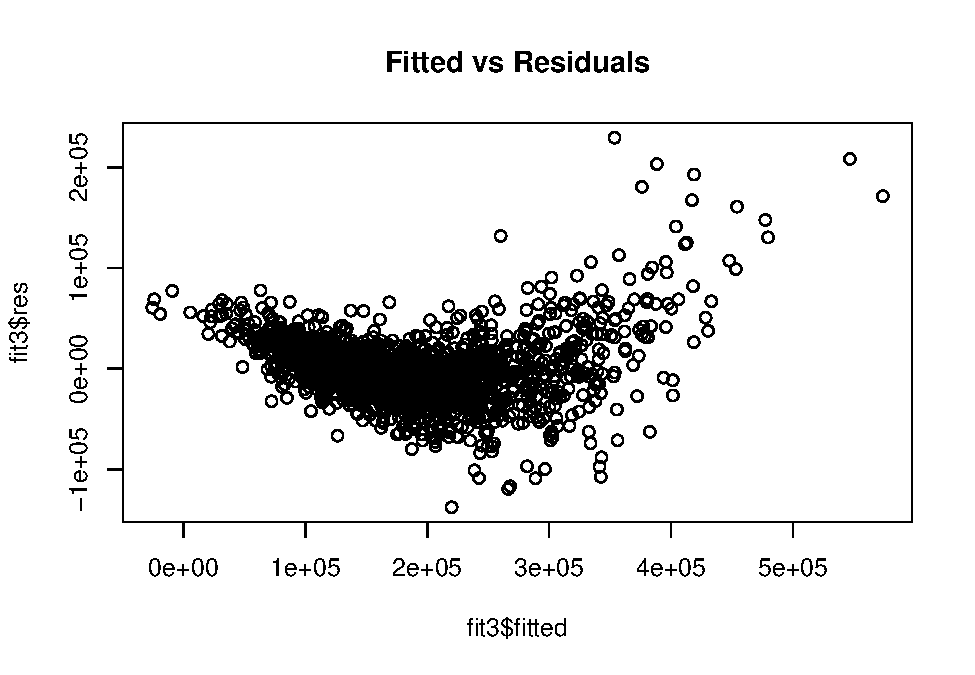
\includegraphics{Predicting-Housing-Price_files/figure-latex/unnamed-chunk-4-1.pdf}

\begin{Shaded}
\begin{Highlighting}[]
\CommentTok{# Check normality of model:}
\KeywordTok{hist}\NormalTok{(fit3}\OperatorTok{$}\NormalTok{res, }\DataTypeTok{main =} \StringTok{"Normality Test"}\NormalTok{,}
     \DataTypeTok{col =} \KeywordTok{c}\NormalTok{(}\StringTok{"blue"}\NormalTok{, }\StringTok{"red"}\NormalTok{, }\StringTok{"green"}\NormalTok{))}
\end{Highlighting}
\end{Shaded}

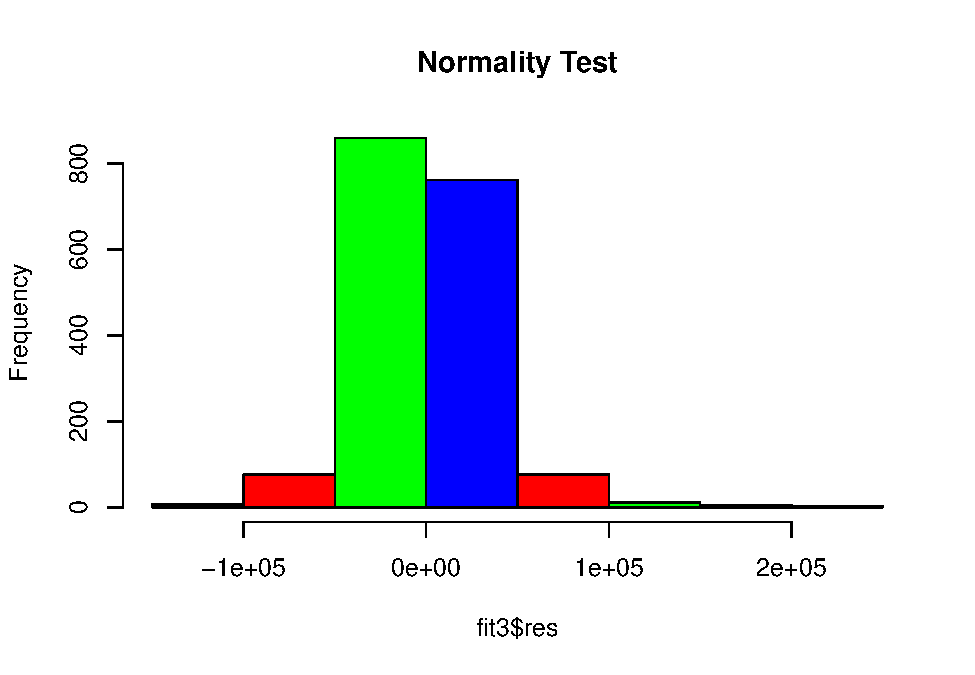
\includegraphics{Predicting-Housing-Price_files/figure-latex/unnamed-chunk-4-2.pdf}

\begin{Shaded}
\begin{Highlighting}[]
\CommentTok{# Plot qq-plot:}
\KeywordTok{qqnorm}\NormalTok{((fit3}\OperatorTok{$}\NormalTok{res))}
\CommentTok{# add reference line:}
\KeywordTok{qqline}\NormalTok{(fit3}\OperatorTok{$}\NormalTok{res)}
\end{Highlighting}
\end{Shaded}

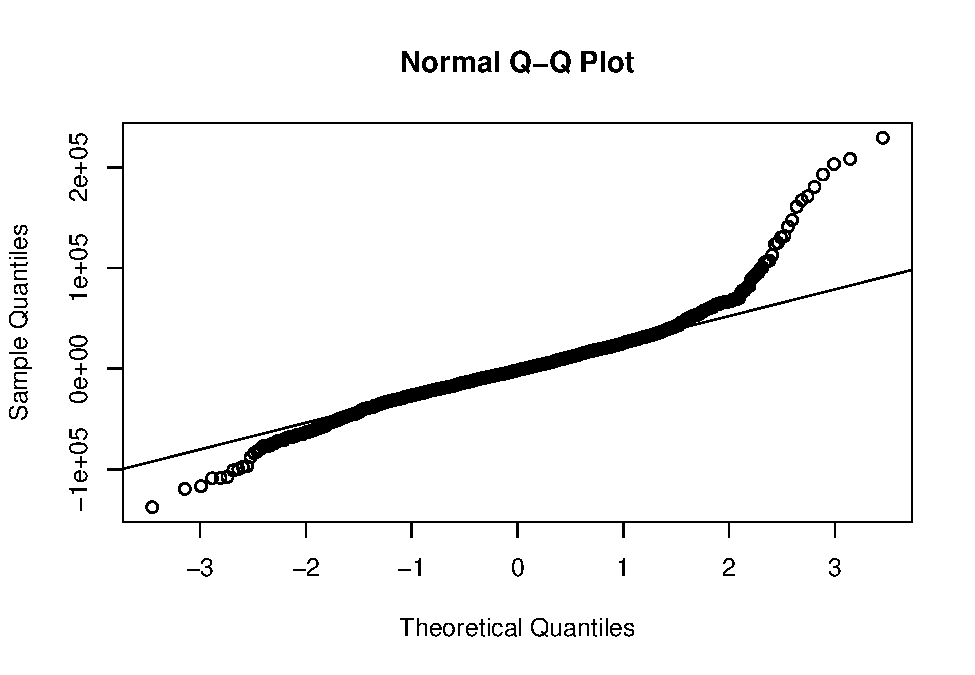
\includegraphics{Predicting-Housing-Price_files/figure-latex/unnamed-chunk-4-3.pdf}

\begin{Shaded}
\begin{Highlighting}[]
\CommentTok{# Compute Shapiro-Wilk Test for Normality Check:}
\KeywordTok{shapiro.test}\NormalTok{(fit3}\OperatorTok{$}\NormalTok{res)}
\end{Highlighting}
\end{Shaded}

\begin{verbatim}
## 
##  Shapiro-Wilk normality test
## 
## data:  fit3$res
## W = 0.93102, p-value < 2.2e-16
\end{verbatim}

\hypertarget{boxcox-transformation}{%
\section{Boxcox Transformation:}\label{boxcox-transformation}}

\begin{Shaded}
\begin{Highlighting}[]
\CommentTok{# Run boxcox transformation to help normalize data:}
\KeywordTok{boxcox}\NormalTok{(SalePrice}\OperatorTok{~}\NormalTok{Overall.Qual }\OperatorTok{+}\StringTok{ }\NormalTok{Year.Built }\OperatorTok{+}\StringTok{ }\NormalTok{Year.Remod.Add }\OperatorTok{+}\StringTok{ }\NormalTok{BsmtFin.SF}\FloatTok{.1} \OperatorTok{+}\StringTok{ }\NormalTok{Total.Bsmt.SF }\OperatorTok{+}\StringTok{ }\NormalTok{X1st.Flr.SF }\OperatorTok{+}\StringTok{ }\NormalTok{Gr.Liv.Area }\OperatorTok{+}\StringTok{ }\NormalTok{TotRms.AbvGrd }\OperatorTok{+}
\StringTok{         }\NormalTok{Garage.Yr.Blt }\OperatorTok{+}\StringTok{ }\NormalTok{Wood.Deck.SF, }\DataTypeTok{data =}\NormalTok{ num.ames)}
\end{Highlighting}
\end{Shaded}

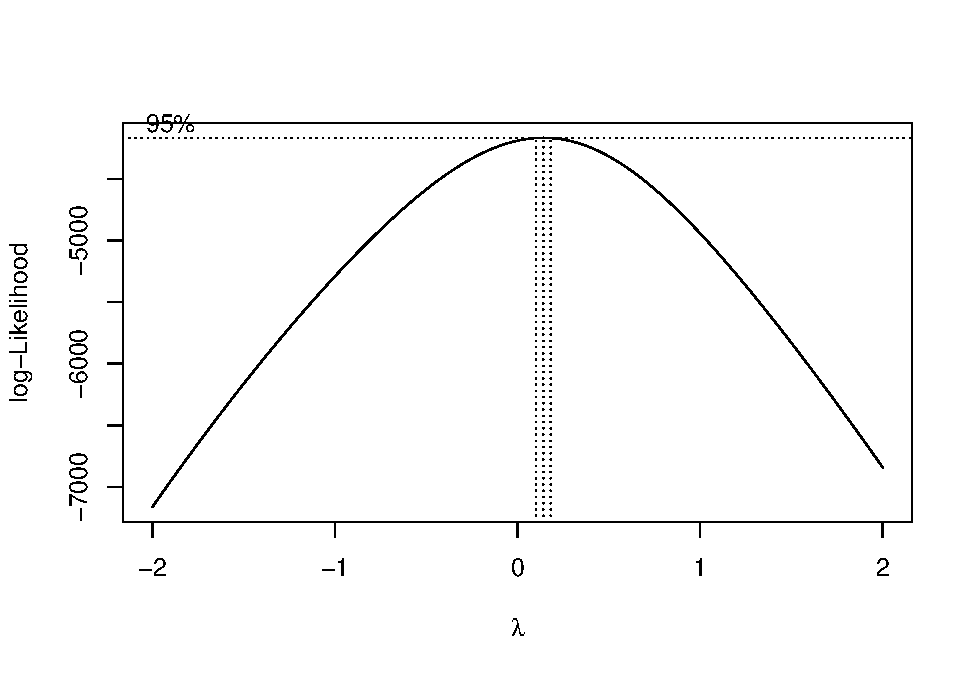
\includegraphics{Predicting-Housing-Price_files/figure-latex/unnamed-chunk-5-1.pdf}

\begin{Shaded}
\begin{Highlighting}[]
\CommentTok{# Create new variable that is the log of SalesPrice:}
\NormalTok{SalePriceLog <-}\StringTok{ }\KeywordTok{log}\NormalTok{(num.ames}\OperatorTok{$}\NormalTok{SalePrice)}

\CommentTok{# Create new model using SalesPriceLog for the dependent variable:}
\NormalTok{fit4 <-}\StringTok{ }\KeywordTok{lm}\NormalTok{(SalePriceLog}\OperatorTok{~}\NormalTok{Overall.Qual }\OperatorTok{+}\StringTok{ }\NormalTok{Year.Built }\OperatorTok{+}\StringTok{ }\NormalTok{Year.Remod.Add }\OperatorTok{+}\StringTok{ }\NormalTok{BsmtFin.SF}\FloatTok{.1} \OperatorTok{+}\StringTok{ }\NormalTok{Total.Bsmt.SF }\OperatorTok{+}\StringTok{ }\NormalTok{X1st.Flr.SF }\OperatorTok{+}\StringTok{ }\NormalTok{Gr.Liv.Area }\OperatorTok{+}\StringTok{ }\NormalTok{TotRms.AbvGrd }\OperatorTok{+}
\StringTok{         }\NormalTok{Garage.Yr.Blt }\OperatorTok{+}\StringTok{ }\NormalTok{Wood.Deck.SF, }\DataTypeTok{data =}\NormalTok{ num.ames)}

\CommentTok{# Plot Fitted vs Residual Values:}
\KeywordTok{plot}\NormalTok{(fit4}\OperatorTok{$}\NormalTok{res}\OperatorTok{~}\NormalTok{fit4}\OperatorTok{$}\NormalTok{fitted, }\DataTypeTok{main =} \StringTok{"Diagnostic Check Model 4"}\NormalTok{)}
\end{Highlighting}
\end{Shaded}

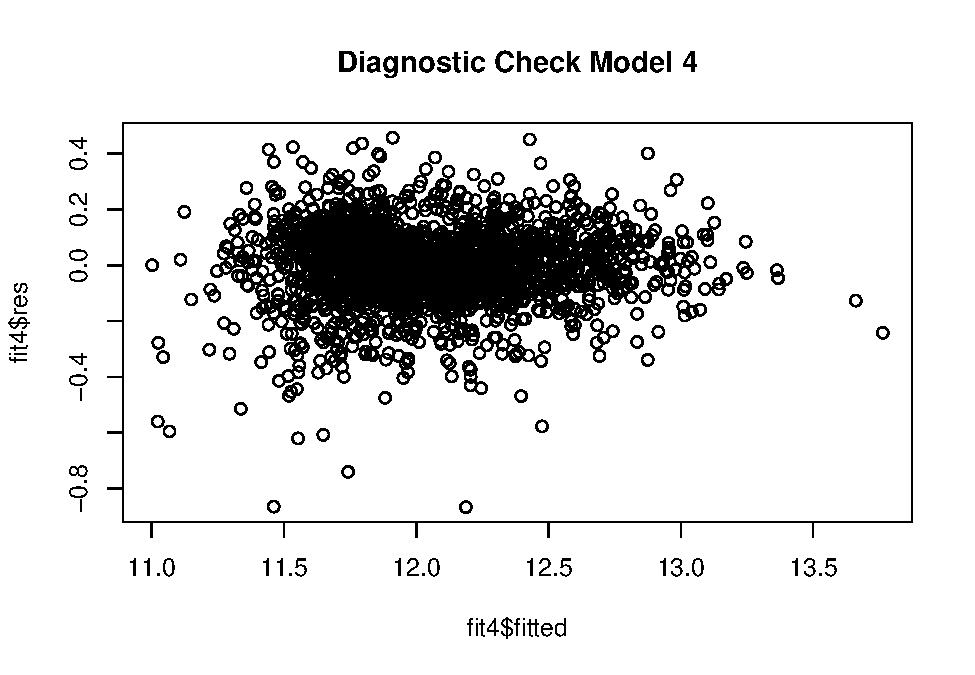
\includegraphics{Predicting-Housing-Price_files/figure-latex/unnamed-chunk-5-2.pdf}
\# Determine Categorical Variables For Model:

\begin{Shaded}
\begin{Highlighting}[]
\CommentTok{# Using anova: determine the categorical variables to use in the final model:}
\NormalTok{model1 =}\StringTok{ }\KeywordTok{lm}\NormalTok{(SalePriceLog }\OperatorTok{~}\StringTok{ }\NormalTok{Overall.Qual }\OperatorTok{+}\StringTok{ }\NormalTok{Year.Built }\OperatorTok{+}\StringTok{ }\NormalTok{Year.Remod.Add }\OperatorTok{+}\StringTok{ }\NormalTok{BsmtFin.SF}\FloatTok{.1} \OperatorTok{+}\StringTok{ }\NormalTok{Total.Bsmt.SF }\OperatorTok{+}\StringTok{ }\NormalTok{X1st.Flr.SF }\OperatorTok{+}\StringTok{ }\NormalTok{Gr.Liv.Area }\OperatorTok{+}\StringTok{ }\NormalTok{Wood.Deck.SF }\OperatorTok{+}\StringTok{ }\NormalTok{Open.Porch.SF, }\DataTypeTok{data =}\NormalTok{ data2, }\DataTypeTok{subset =}\NormalTok{ train)}
\NormalTok{model2 =}\StringTok{ }\KeywordTok{lm}\NormalTok{(SalePriceLog }\OperatorTok{~}\StringTok{ }\NormalTok{Overall.Qual }\OperatorTok{+}\StringTok{ }\NormalTok{Year.Built }\OperatorTok{+}\StringTok{ }\NormalTok{Year.Remod.Add }\OperatorTok{+}\StringTok{ }\NormalTok{BsmtFin.SF}\FloatTok{.1} \OperatorTok{+}\StringTok{ }\NormalTok{Total.Bsmt.SF }\OperatorTok{+}\StringTok{ }\NormalTok{X1st.Flr.SF }\OperatorTok{+}\StringTok{ }\NormalTok{Gr.Liv.Area }\OperatorTok{+}\StringTok{ }\NormalTok{Wood.Deck.SF }\OperatorTok{+}\StringTok{ }\NormalTok{Open.Porch.SF }\OperatorTok{+}\StringTok{ }\NormalTok{Street, }\DataTypeTok{data =}\NormalTok{ data2, }\DataTypeTok{subset =}\NormalTok{ train)}
\KeywordTok{anova}\NormalTok{(model1,model2)}
\end{Highlighting}
\end{Shaded}

\begin{verbatim}
## Analysis of Variance Table
## 
## Model 1: SalePriceLog ~ Overall.Qual + Year.Built + Year.Remod.Add + BsmtFin.SF.1 + 
##     Total.Bsmt.SF + X1st.Flr.SF + Gr.Liv.Area + Wood.Deck.SF + 
##     Open.Porch.SF
## Model 2: SalePriceLog ~ Overall.Qual + Year.Built + Year.Remod.Add + BsmtFin.SF.1 + 
##     Total.Bsmt.SF + X1st.Flr.SF + Gr.Liv.Area + Wood.Deck.SF + 
##     Open.Porch.SF + Street
##   Res.Df    RSS Df Sum of Sq     F    Pr(>F)    
## 1   1790 33.184                                 
## 2   1789 32.960  1   0.22384 12.15 0.0005028 ***
## ---
## Signif. codes:  0 '***' 0.001 '**' 0.01 '*' 0.05 '.' 0.1 ' ' 1
\end{verbatim}

\begin{Shaded}
\begin{Highlighting}[]
\KeywordTok{str}\NormalTok{(data2)}
\end{Highlighting}
\end{Shaded}

\begin{verbatim}
## 'data.frame':    2258 obs. of  74 variables:
##  $ MS.Zoning      : chr  "RL" "RH" "RL" "RL" ...
##  $ Lot.Frontage   : int  141 80 81 93 74 78 41 43 39 60 ...
##  $ Lot.Area       : int  31770 11622 14267 11160 13830 9978 4920 5005 5389 7500 ...
##  $ Street         : chr  "Pave" "Pave" "Pave" "Pave" ...
##  $ Alley          : chr  "None" "None" "None" "None" ...
##  $ Lot.Shape      : chr  "IR1" "Reg" "IR1" "Reg" ...
##  $ Land.Contour   : chr  "Lvl" "Lvl" "Lvl" "Lvl" ...
##  $ Lot.Config     : chr  "Corner" "Inside" "Corner" "Corner" ...
##  $ Land.Slope     : chr  "Gtl" "Gtl" "Gtl" "Gtl" ...
##  $ Condition.1    : chr  "Norm" "Feedr" "Norm" "Norm" ...
##  $ Condition.2    : chr  "Norm" "Norm" "Norm" "Norm" ...
##  $ Bldg.Type      : chr  "1Fam" "1Fam" "1Fam" "1Fam" ...
##  $ House.Style    : chr  "1Story" "1Story" "1Story" "1Story" ...
##  $ Overall.Qual   : int  6 5 6 7 5 6 8 8 8 7 ...
##  $ Overall.Cond   : int  5 6 6 5 5 6 5 5 5 5 ...
##  $ Year.Built     : int  1960 1961 1958 1968 1997 1998 2001 1992 1995 1999 ...
##  $ Year.Remod.Add : int  1960 1961 1958 1968 1998 1998 2001 1992 1996 1999 ...
##  $ Roof.Style     : chr  "Hip" "Gable" "Hip" "Hip" ...
##  $ Roof.Matl      : chr  "CompShg" "CompShg" "CompShg" "CompShg" ...
##  $ Exterior.1st   : chr  "BrkFace" "VinylSd" "Wood" "BrkFace" ...
##  $ Exterior.2nd   : chr  "Plywood" "VinylSd" "wood" "BrkFace" ...
##  $ Mas.Vnr.Type   : chr  "Stone" "None" "BrkFace" "None" ...
##  $ Mas.Vnr.Area   : int  112 0 108 0 0 20 0 0 0 0 ...
##  $ Exter.Qual     : chr  "TA" "TA" "TA" "Gd" ...
##  $ Exter.Cond     : chr  "TA" "TA" "TA" "TA" ...
##  $ Foundation     : chr  "CBlock" "CBlock" "CBlock" "CBlock" ...
##  $ Bsmt.Qual      : chr  "TA" "TA" "TA" "TA" ...
##  $ Bsmt.Cond      : chr  "Gd" "TA" "TA" "TA" ...
##  $ Bsmt.Exposure  : chr  "Gd" "No" "No" "No" ...
##  $ BsmtFin.Type.1 : chr  "BLQ" "Rec" "ALQ" "ALQ" ...
##  $ BsmtFin.SF.1   : int  639 468 923 1065 791 602 616 263 1180 0 ...
##  $ BsmtFin.Type.2 : chr  "Unf" "LwQ" "Unf" "Unf" ...
##  $ BsmtFin.SF.2   : int  0 144 0 0 0 0 0 0 0 0 ...
##  $ Bsmt.Unf.SF    : int  441 270 406 1045 137 324 722 1017 415 994 ...
##  $ Total.Bsmt.SF  : int  1080 882 1329 2110 928 926 1338 1280 1595 994 ...
##  $ Heating        : chr  "Gas" "Gas" "Gas" "Gas" ...
##  $ Heating.QC     : chr  "Fa" "TA" "TA" "Ex" ...
##  $ Central.Air    : chr  "Y" "Y" "Y" "Y" ...
##  $ Electrical     : chr  "SBrkr" "SBrkr" "SBrkr" "SBrkr" ...
##  $ X1st.Flr.SF    : int  1656 896 1329 2110 928 926 1338 1280 1616 1028 ...
##  $ X2nd.Flr.SF    : int  0 0 0 0 701 678 0 0 0 776 ...
##  $ Low.Qual.Fin.SF: int  0 0 0 0 0 0 0 0 0 0 ...
##  $ Gr.Liv.Area    : int  1656 896 1329 2110 1629 1604 1338 1280 1616 1804 ...
##  $ Bsmt.Full.Bath : int  1 0 0 1 0 0 1 0 1 0 ...
##  $ Bsmt.Half.Bath : int  0 0 0 0 0 0 0 0 0 0 ...
##  $ Full.Bath      : int  1 1 1 2 2 2 2 2 2 2 ...
##  $ Half.Bath      : int  0 0 1 1 1 1 0 0 0 1 ...
##  $ Bedroom.AbvGr  : int  3 2 3 3 3 3 2 2 2 3 ...
##  $ Kitchen.AbvGr  : int  1 1 1 1 1 1 1 1 1 1 ...
##  $ Kitchen.Qual   : chr  "TA" "TA" "Gd" "Ex" ...
##  $ TotRms.AbvGrd  : int  7 5 6 8 6 7 6 5 5 7 ...
##  $ Functional     : chr  "Typ" "Typ" "Typ" "Typ" ...
##  $ Fireplaces     : int  2 0 0 2 1 1 0 0 1 1 ...
##  $ Fireplace.Qu   : chr  "Gd" "None" "None" "TA" ...
##  $ Garage.Type    : chr  "Attchd" "Attchd" "Attchd" "Attchd" ...
##  $ Garage.Yr.Blt  : int  1960 1961 1958 1968 1997 1998 2001 1992 1995 1999 ...
##  $ Garage.Finish  : chr  "Fin" "Unf" "Unf" "Fin" ...
##  $ Garage.Cars    : int  2 1 1 2 2 2 2 2 2 2 ...
##  $ Garage.Area    : int  528 730 312 522 482 470 582 506 608 442 ...
##  $ Garage.Qual    : chr  "TA" "TA" "TA" "TA" ...
##  $ Garage.Cond    : chr  "TA" "TA" "TA" "TA" ...
##  $ Paved.Drive    : chr  "P" "Y" "Y" "Y" ...
##  $ Wood.Deck.SF   : int  210 140 393 0 212 360 0 0 237 140 ...
##  $ Open.Porch.SF  : int  62 0 36 0 34 36 0 82 152 60 ...
##  $ Enclosed.Porch : int  0 0 0 0 0 0 170 0 0 0 ...
##  $ X3Ssn.Porch    : int  0 0 0 0 0 0 0 0 0 0 ...
##  $ Screen.Porch   : int  0 120 0 0 0 0 0 144 0 0 ...
##  $ Pool.Area      : int  0 0 0 0 0 0 0 0 0 0 ...
##  $ Fence          : chr  "None" "MnPrv" "None" "None" ...
##  $ Misc.Val       : int  0 0 12500 0 0 0 0 0 0 0 ...
##  $ Yr.Sold        : int  2010 2010 2010 2010 2010 2010 2010 2010 2010 2010 ...
##  $ Sale.Type      : chr  "WD " "WD " "WD " "WD " ...
##  $ Sale.Condition : chr  "Normal" "Normal" "Normal" "Normal" ...
##  $ SalePrice      : int  215000 105000 172000 244000 189900 195500 213500 191500 236500 189000 ...
##  - attr(*, "na.action")= 'omit' Named int [1:667] 12 15 23 24 25 28 56 58 59 67 ...
##   ..- attr(*, "names")= chr [1:667] "12" "15" "23" "24" ...
\end{verbatim}

\end{document}
